\documentclass[12pt]{article}
\usepackage{amsfonts}
\usepackage{amsmath}
\usepackage{graphicx}
\setcounter{tocdepth}{2}
\usepackage{xcolor}
\newtheorem{proposition}{Proposition}
\newtheorem{lemma}{Lemma}
\newcommand{\blue}[1]{\textcolor{blue}{#1}}
\usepackage{float}
\usepackage[caption = false]{subfig}
\usepackage{/Users/timbarry/optionFiles/mymacros}
\DeclareMathOperator*{\argmin}{arg\,min}

\begin{document}
\noindent
Tim, Gene, Kathryn
\begin{center}
\textbf{CRISPR genome editing, single-cell sequencing, and exponential family measurement error models}
\end{center}

\begin{abstract}
CRISPR genome engineering and single-cell sequencing have transformed biological discovery. Single-cell CRISPR screens unite these two technologies, linking genetic perturbations in individual cells to changes in gene expression and illuminating regulatory networks underlying diseases. In this work we study single-cell CRISPR screens from a statistical perspective. First, we demonstrate on real data that a standard method for estimation and inference in single-cell CRISPR screens — “thresholded regression” — exhibits attenuation bias and a bias-variance tradeoff as a function of an intrinsic tuning parameter. We recover these phenomena in precise theoretical terms in an idealized Gaussian setting. Next, we introduce GLM-EIV (“generalized linear model with errors-in-variables”), a new method for single-cell CRISPR screen analysis. GLM-EIV generalizes the classical errors-in-variables model to response distributions and sources of measurement error that are exponential family-distributed, overcoming limitations of thresholded regression. We develop a computational infrastructure to deploy GLM-EIV across hundreds or thousands of processors on clouds (e.g., Microsoft Azure) and high-performance clusters. Leveraging this infrastructure, we apply GLM-EIV to analyze two recent, large-scale, single-cell CRISPR screen datasets, yielding new biological insights.
\end{abstract}

\tableofcontents

\section{Introduction}
CRISPR is a genome engineering tool that has enabled scientists to precisely edit human and nonhuman genomes, opening the door to new medical therapies \cite{Rothgangl2021,Musunuru2021} and transforming basic biology research \cite{Przybyla2021}. Recently, scientists have paired CRISPR genome engineering with single-cell sequencing \cite{Dixit2016,Datlinger2017}. The resulting assays, known as a ``single-cell CRISPR screens,'' link genetic perturbations in individual cells to changes in gene expression, illuminating regulatory networks underlying human diseases and other traits \cite{Morris2021a}.

Despite their promise, single-cell CRISPR screens present substantial statistical challenges. A major difficulty is that CRISPR perturbations are unobservable and assigned stochastically to cells. As a consequence, one cannot know with certainty which cells were perturbed. Instead, one must leverage an indirect, noisy proxy of perturbation presence or absence -- namely, transcribed barcode counts -- to ``guess'' which cells were perturbed. Using these imputed perturbation assignments, one can attempt to estimate the effect of the perturbation on gene expression. The standard approach, which we call ``thresholded regression'' or the ``thresholding method,'' is to assign perturbation identities to cells by simply thresholding the barcode counts.

We study estimation and inference in single-cell CRISPR screens from a statistical perspective, formulating the data generating mechanism using a new class of errors-in-variables (or measurement error) models. We assume that the response variable $y$ is a GLM of an underlying predictor variable $x^*$. We do not observe $x^*$ directly; rather, we observe a noisy version $x$ of $x^*$ that itself is a GLM of $x^*$. The goal of the analysis is to estimate the effect of $x^*$ on $y$ using the observed data $(x , y)$ only. In the context of the biological application, $x^*$, $y$, and $x$ are CRISPR perturbations, gene expressions, and barcode counts, respectively.

Our work makes two main contributions. First, we conduct an investigation of the thresholding method from empirical and theoretical perspectives. Notably, we demonstrate on real data that the thresholding method exhibits attenuation bias and a bias-variance tradeoff as a function of the selected threshold, and we recover these phenomena in precise mathematical terms in an idealized Gaussian model. Second, we introduce a new method for estimation and inference in single-cell CRISPR screens that accounts for the measurement error inherent in the experiment. The method, called \textit{GLM-EIV} (generalized linear model with errors-in-variables), implicitly estimates the probability that each cell was perturbed, obviating the need to explicitly impute perturbation assignments via thresholding or another heuristic. Theoretical analyses and simulation studies indicate that GLM-EIV outperforms the thresholding method in large regions of the parameter space.

We implement several statistical accelerations (that likely are of independent utility) to bring the cost of GLM-EIV down to within an order of magnitude of the thresholding method. Finally, we develop a computational infrastructure to deploy GLM-EIV at-scale across hundreds or thousands of processors on clouds (e.g., Microsoft Azure) and high-performance clusters. Leveraging this infrastructure, we apply GLM-EIV to analyze two recent, large-scale, high multiplicity-of-infection single-cell CRISPR screen datasets, yielding new biological and statistical insights. 

\section{Background and analysis challenges}

Our focus in this work is on high multiplicity-of-infection (MOI), enhancer-targeting, single-cell CRISPR screens. In this section we cover relevant biological background and motivation.
\\ \\
\textbf{P1}: The human genome consists of genes (segments of DNA that code for proteins), enhancers (segments of DNA that regulate the expression of one or more genes), and other genomic regions. Genome-wide association studies have revealed that the majority ($>95\%$) of variants associated with diseases lie outside genes and (very likely) inside enhancers. These noncoding variants contribute to disease by modulating the expression one or more genes, which in turn encode proteins that affect the phenotype. A central open challenge in genetics, therefore, is to link enhancers that harbor disease-associated variants to the genes that they target at genome-wide scale.
\\ \\
\textbf{P2}: High MOI single-cell CRISPR screens are the most promising biotechnology for solving this problem. \blue{Describe the experimental protocol here. Explain that we use the terms ``barcodes'' and ``gRNAs'' interchangeably, as polyadenylated gRNAs serve as barcodes in CROP-seq. Link to Figure \ref{analysis_challenges}.}
\\ \\
\textbf{P3}: Single-cell CRISPR screens pose several core analysis challenges. \blue{Describe the analysis challenges here: (i) unobserved perturbation; (ii) existence of background reads; (iii) highly discrete count data; (iv) nuisance variables}.

\begin{figure}[h!]
	\centering
	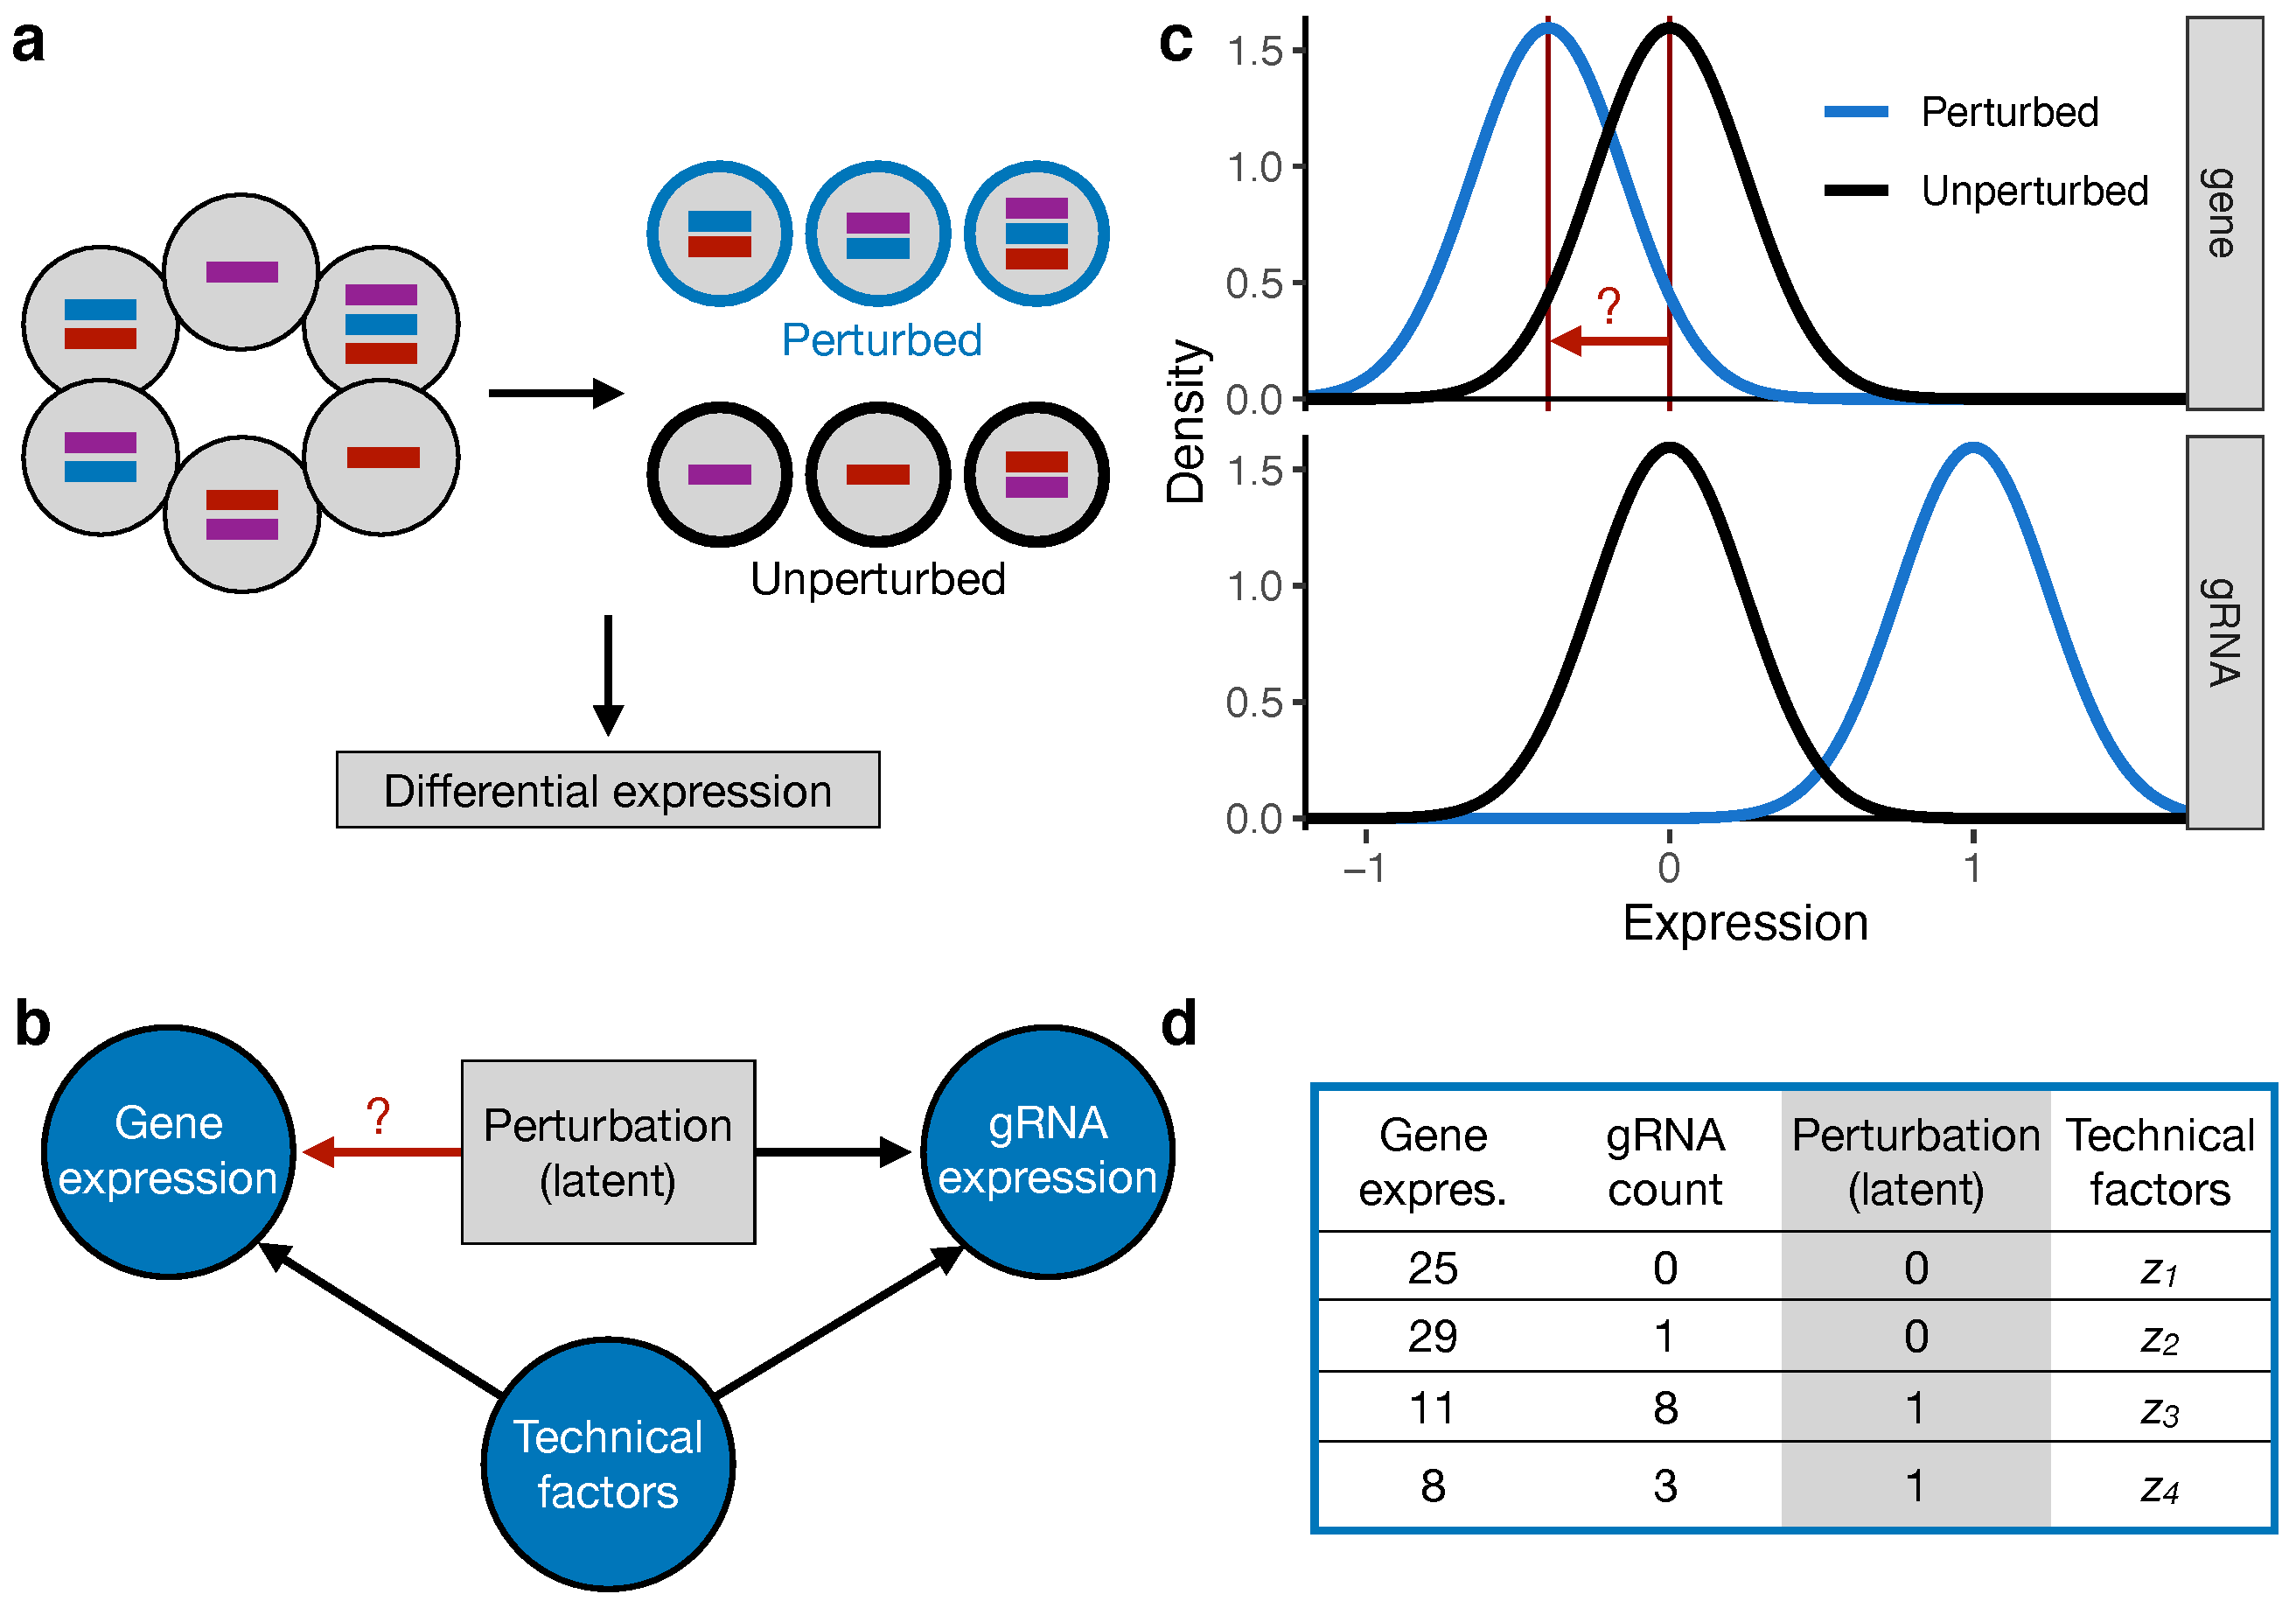
\includegraphics[width=1\linewidth]{../../figures/analysis_challenges/plot.pdf}
	\caption{\textbf{Experimental design and analysis challenges}: \textbf{a,} Experimental design. For a given perturbation (e.g., the perturbation represented in yellow), we partition the cells into two groups: those that received the perturbation, and those that did not receive the perturbation. For a given gene, we conduct a differential expression analysis across the two groups of cells, yielding an estimate of the impact of the given perturbation on the given gene. \textbf{b,} DAG representing the variables in the analysis. The perturbation (unobserved) affects both gene expression and gRNA expression; technical factors (e.g., batch, sequencing depth, etc.) act as nuisance variables. The target of inference is the effect of the perturbation on gene expression (denoted with question mark). \textbf{c,} Schematic illustrating ``background reads.'' The gRNA modality has a nonzero, ``background read'' distribution even in the absence of a perturbation, complicating the assignment of perturbations to cells. \textbf{d}, Example data for a given perturbation-gene pair. Notice that (i) the perturbations are unobserved, and (ii) the gene and gRNA expression data take the form of discrete counts.}
	\label{analysis_challenges}
\end{figure}

\section{Related work}

Motivated by the challenges of single-cell data, several authors recently have extended statistical models that (implicitly or explicitly) assume Gaussianity and homoscedasticity to a broader class of exponential family distributions. For example, Lin, Lei, and Roeder \cite{Lin2021} developed eSVD, an extension of SVD to exponential family and curved Gaussian responses. Unlike SVD, eSVD models the relationship between the mean and variance of a gene's expression level, a phenomenon induced by the countedness of single-cell data \cite{Lause2021}.
Similarly, Townes et al.\ \cite{Townes2019} proposed GLM-PCA, an extension of PCA that directly models Poisson- or negative binomially-distributed gene expression counts. We see our work as a continuation of this broad effort to ``port'' common statistical methods and models to single-cell count data. Our focus, however, is on regression rather than dimension reduction: we extend the classical errors-in-variables model to response distributions and sources of measurement error that are exponential family-distributed.

The closest parallels to our work in the statistical methodology literature are Gr\"{u}n \& Leisch \cite{Grun2008} and Ibrahim \cite{Ibrahim1990}. Gr\"{u}n \& Leisch considered estimation and inference in a $k$-component mixture of GLMs. While we prefer to view the GLM-EIV model as an errors-in-variables model,  the GLM-EIV model is equivalent to a two-component mixture of \textit{products} of GLM densities. Ibrahim derived a method for fitting GLMs in the presence of missing-at-random covariates. Our method, by contrast, involves fitting two conditionally independent GLMs in the presence of a totally latent covariate. Thus, while Ibrahim is a helpful reference, our estimation and inference tasks are more complex.

The genomics literature has produced several applied methods for linking perturbations to changes in gene expression in single-cell CRISPR screens: SCEPTRE \cite{Barry2020}, MIMOSCA \cite{Dixit2016}, and scMAGeCK \cite{Yang2019}. These methods in general are focused on hypothesis testing rather than estimation; none, for instance, produces a confidence interval for the effect size of a perturbation on gene expression change. Additionally, two of these methods (MIMOSCA and scMAGeCK) use (possibly penalized) linear models to model gene expressions, thereby disregarding the countedness and sparsity of the data. 

\section{Thresholding method}

In this section we study thresholded regression from empirical and theoretical perspectives, highlighting several limitations of the method. Let $n \in \N$ be the number of cells assayed in the experiment (typically, $n \approx 100,000 - 250,000$). Consider a single perturbation and a single gene. For cell $i \in \{1, \dots, n\}$, let $m_i \in \N$ be the number of gene transcripts sequenced in the cell; let $g_i \in \N$ be the number of gRNA transcripts sequenced in the cell; let $l^m_i \in \N$ be the number of gene transcripts sequenced across \textit{all} genes (the library size) in the cell; and finally, let $z_i \in \R^{d-1}$ be the cell-specific vector of technical factors (e.g., sequencing batch, percent mitochondrial reads, etc.). The thresholding method is defined as follows:
\begin{itemize}
\item[1.] For a given threshold $c \in \N$, let the imputed perturbation assignment $\hat{p}_i \in \{0, 1\}$ be $$\begin{cases} \hat{p}_i = 0 \textrm{ if } g_i \geq c, \\ \hat{p}_i = 1 \textrm{ if } g_i < c. \end{cases}$$
\item[2.] Assume that $m_i$ is related to $\hat{p}_i, l_i,$ and $z_i$ through the following GLM:
\begin{equation*}
\begin{cases}
m_i | (\hat{p}_i, z_i, l_i) \sim \textrm{NB}_\theta(\mu_i), \\
\log(\mu_i) = \beta^m_0 + \beta^m_1 \hat{p}_i + \gamma^T_m z_i + \log\left( l_i^m\right),
\end{cases}
\end{equation*}
where (i) $NB_\theta(\mu_i)$ is a negative binomial distribution with mean $\mu_i$ and known size parameter $\theta$; (ii) $\beta^m_0 \in \R, \beta^m_1 \in \R,$ and $\gamma \in  \R^{d-1}$ are unknown parameters; and (iii) $\log(l_i^m)$ is an offset term. Fit a GLM to obtain estimates of the parameters.

\item[3.] Compute a $p$-value and confidence interval for the target of inference $\beta^m_1$.
\end{itemize}

The biological interpretation for the target of inference $\beta^m_1$ as follows:  $\beta^m_1$ is the log-transformed fold change in gene expression in response to the perturbation, removing the effect of the technical factors. Fold change (obtained by exponentiating $\beta^m_1$) is the ratio of the mean expression in cells that were perturbed to the mean expression in cells that were not perturbed. $\exp(\beta^m_1) = 1$ indicates no change in mean expression, while $\exp(\beta^m_1) > 1$ and $\exp(\beta^m_1) < 1$ indicate an increase and decrease in expression in response to the perturbation, respectively (accounting for technical factors).

\subsection{Empirical analysis}

We examined the behavior of the thresholding method on real data and uncovered attenuation bias and bias-variance tradeoff effects. We applied the thresholding method to analyze the set of 381 positive control perturbation-gene pairs in the Gasperini dataset. The positive control pairs consisted of perturbations that targeted gene transcription start sites (TSSs) for inhibition. Repressing the TSS of a given gene decreases its expression; therefore, the positive control pairs \textit{a priori} are expected to exhibit a strong, negative log fold change in expression.

To investigate the sensitivity of the thresholding method to the selected threshold, we deployed the thresholding method on the positive control data using three different thresholds: 1, 5, and 20. We found that the chosen threshold substantially impacted the results (Figure \ref{thresholding_empirical}a-b). Estimates for log fold change produced by threshold = 1 were smaller in magnitude than those produced by threshold = 5. (Equivalently, estimates for \textit{raw} fold change were closer to the baseline of $1$ for threshold = 1; Figure \ref{thresholding_empirical}a.) Estimates produced by threshold = 5 and threshold = 20 were more concordant, but threshold = 20 yielded slightly larger effect sizes (Figure \ref{thresholding_empirical}b).

We reasoned that thresholded regression underestimated effect sizes on the positive control pairs, especially for threshold = 1 (an example of \textit{attenuation bias}). For a given perturbation, the vast majority ($>99\%$) of cells are unperturbed. This imbalance leads to an asymmetry: misclassifying \textit{unperturbed} cells as \textit{perturbed} is intuitively ``worse'' than misclassifying \textit{perturbed} cells as \textit{unperturbed}. Misclassified \textit{unperturbed} cells contaminate the set of truly perturbed cells, leading to attenuation bias; by contrast, misclassified \textit{perturbed} cells are swamped in number and ``neutralized'' by the truly \textit{unperturbed} cells. Setting the threshold to a large number reduces the unperturbed-to-perturbed misclassification rate, decreasing bias.

We hypothesized, however, that the reduction in bias conferred by selecting a large threshold incurs the cost of increasing the variance of the estimator. To investigate, we compared $p$-values and confidence intervals produced by threshold = 5 and threshold = 20 for the target of inference $\beta^m_1$. We found that threshold = 5 yielded smaller (i.e., more significant) $p$-values and narrower confidence intervals than did threshold = 20 (Figure \ref{thresholding_empirical}c-d). We concluded that thresholded regression has a bias-variance tradeoff: as the threshold increases, bias decreases and variance increases.

Finally, to determine whether there is an ``obvious'' location at which to draw the threshold, we examined the empirical gRNA count distributions and checked for bimodality. Figures \ref{thresholding_empirical}e and \ref{thresholding_empirical}f display the empirical distribution of a randomly-selected gRNA from the Gasperini and Xie datasets, respectively (counts of $0$ omitted). The distributions peak at $1$ and then taper off gradually; there does not exist a sharp boundary that cleanly separates the perturbed from the unperturbed cells. Overall, we concluded that the thresholding method faces several challenges: (i) the threshold is a tuning parameter that significantly impacts the results; (ii) the threshold mediates an intrinsic bias-variance tradeoff; and (iii) the gRNA count distributions do not imply a clear threshold selection strategy.

\begin{figure}[h!]
	\centering
	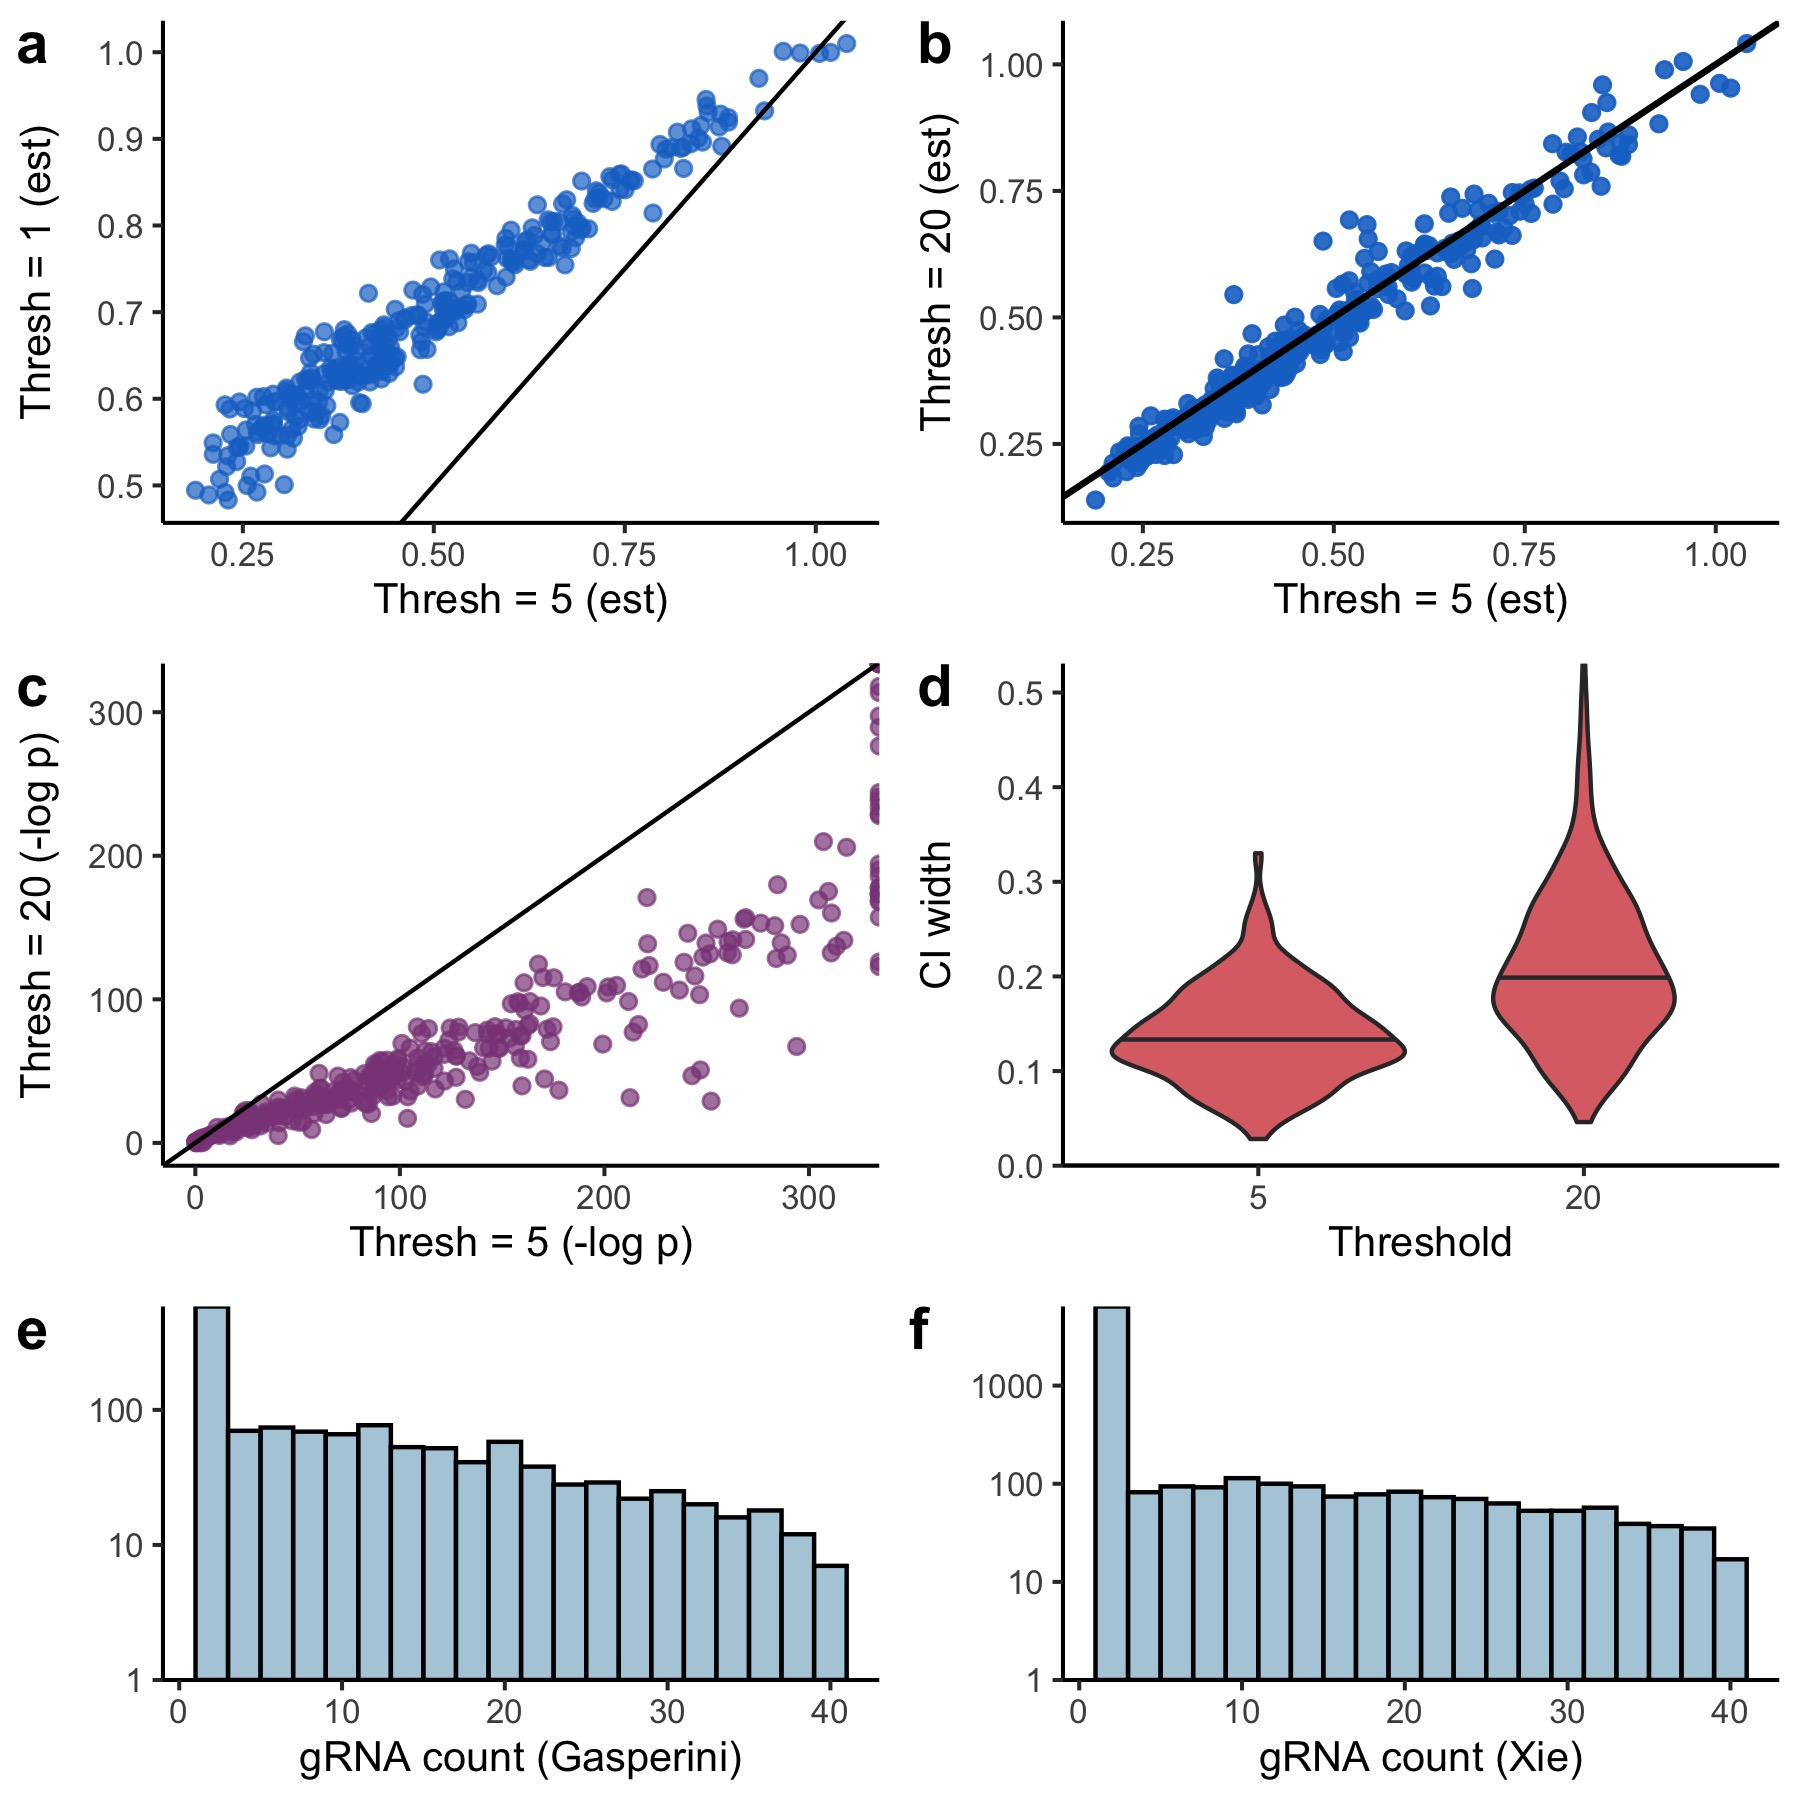
\includegraphics[width=1\linewidth]{../../figures/thresholding_empirical/plot}
	\caption{\textbf{Empirical challenges of thresholded regression.} \textbf{a-b,} Fold change estimates produced by threshold = 1 versus threshold = 5 (a) and threshold = 20 versus threshold = 5 (b). The selected threshold substantially impacts the results. \textbf{c-d,} $p$-values (c) and CI widths (d) produced by threshold = 20 versus threshold = 5. The latter threshold yields more confident estimates. \textbf{e-f}, Empirical distribution of randomly-selected gRNA from Gasperini (e) and Xie (f) data. The gRNA data do not appear to imply an obvious threshold selection strategy.}
	\label{thresholding_empirical}
\end{figure}
\newpage

\subsection{Theoretical analysis}\label{sec:thresholding_theory}

We study the thresholding method from a theoretical perspective in an idealized Gaussian setting. Suppose that we observe data $(g_1, m_1), \dots, (g_n, m_n)$ from the following model:

\begin{equation}\label{theoretical_model}
\begin{cases}
m_i = \beta^m_0 + \beta^m_1 p_i + \ep_i \\
g_i = \beta^g_0 + \beta^g_1 p_i + \tau_i \\
p_i \sim \textrm{Bern}(\pi) \\
\ep_i, \tau_i \sim N(0,1) \\
p_i \indep \tau_i \indep \ep_i.
\end{cases}
\end{equation}
For a given threshold $c \in \R$, the imputed perturbation assignment $\hat{p}_i$ is given by $\hat{p}_i = \mathbb{I}(g_i \geq c).$ The thresholding estimator $\hat{\beta}^m_1$ for $\beta^m_1$ is $$\hat{\beta}^m_1 = \frac{\sum_{i=1}^n (\hat{p}_i - \overline{\hat{p}}) (m_i - \overline{m})}{\sum_{i=1}^n (\hat{p}_i - \overline{\hat{p}})^2 }.$$

\begin{proposition}\label{prop:convergence}
 The almost sure limit (as $n \to \infty$) of $\hat{\beta}^m_1$ is
\begin{equation}\label{thresh_est_intercepts}
\hat{\beta}^m_1 \xrightarrow{a.s.} \beta^m_1 \left(\frac{ \pi( \omega - \E[ \hat{p}_i ])}{ \E[\hat{p}_i] (1 - \E[\hat{p}_i])}\right),
\end{equation}
where
$$\begin{cases}
\E[\hat{p}_i] = \zeta(1-\pi) + \omega\pi , \\
\omega = \Phi\left(\beta_1^g + \beta_0^g -c \right) ,\\ \zeta = \Phi\left( \beta^g_0 - c \right). \\
\end{cases}$$
\end{proposition}
Let $\gamma: \R^4 \to \R$ be defined by
$$ \gamma(\beta^g_1, \pi, c, \beta^g_0) = \frac{\pi (\omega - \E[\hat{p}_i])}{\E[\hat{p}_i] (1 - \E[\hat{p}_i]) }.$$ We call $\gamma$ the ``attenuation function.'' Observe that \begin{itemize}
\item[i.] $\gamma$ does not depend on $\beta^m_1$ or $\beta^m_0$, and
\item[ii.] $\hat{\beta}^m_1 \xrightarrow{a.s.} [\gamma(\beta_0^g, \beta_1^g, c, \pi)] \beta^m_1.$
\end{itemize}
Let $b: \R^4 \to \R$ be the asymptotic \textit{relative} bias of $\hat{\beta}^m_1$:
\begin{multline*}
b(\beta^g_1, \pi, c, \beta^g_0) = \left(\frac{1}{\beta^m_1}\right) \lim_{n\to\infty} \left(\beta^m_1 - \E[\hat{\beta}^m_1]\right) = \left( \frac{1}{\beta^m_1}\right)\left(\beta^m_1 - \E \left(\lim_{a.s.} \hat{\beta}^m_1 \right)\right) \\ = \frac{1}{\beta^m_1} \left(\beta^m_1 - \gamma(\beta^g_1, \pi, c, \beta^g_0)\beta^m_1\right) = 1 - \gamma(\beta^g_1, \pi, c, \beta^g_0),
\end{multline*}
where $\lim_{a.s.}$ denotes a.s.\ convergence. The asymptotic relative bias vanishes when the attenuation function equals $1$. \textcolor{red}{(HOW TO MAKE THE ABOVE RIGOROUS?)}

\begin{center}
\textbf{Bias as a function of threshold (Panel a)}
\end{center}

To investigate the basic question of ``What is a good threshold selection strategy?'', we study the relationship between the asymptotic relative bias $b$ of $\hat{\beta}^m_1$ and the selected threshold $c$. For simplicity, we set the perturbation probability $\pi$ to $1/2$. Let $c_\textrm{bayes} \in \R$ be the Bayes-optimal decision boundary for classifying cells as perturbed or unperturbed, i.e. $$c_\textrm{bayes} = \argmin_{c \in \R} \P(\hat{p}_i \neq p_i).$$ Simple algebra shows that $c_\textrm{bayes} = \beta_0^g + (1/2) \beta^g_1.$ Below, we give several results for the asymptotic relative bias $b$ of $\hat{\beta}^m_1$. We refer throughout to Figure \ref{thresholding_theoretical}a, which displays plots of asymptotic relative bias versus threshold for different values of $\beta^g_1$. We sometimes refer to ``asymptotic relative bias'' using the shortened term ``bias'' for succinctness.

\begin{itemize}
\item 
\begin{proposition}\label{prop:att_bias} Fix $\pi = 1/2$. For all $(\beta^g_1, c, \beta^g_0) \in \R^3$, the asymptotic relative bias is positive, i.e. 
$$b(\beta^g_1, 1/2, c, \beta^g_0) > 0.$$
\end{proposition}
The thresholding method incurs strict attenuation bias (i.e., it \textit{under}estimates the true effect size) for all choices of the threshold and over all possible values of the model parameters (Figure \ref{thresholding_theoretical}a). Attenuation bias is a common attribute of estimators that ignore measurement in errors-in-variables models \cite{Stefanski2000a}.
\item
\begin{proposition}\label{prop:monotonic} Fix $\pi = 1/2$. The asymptotic relative bias $b$ decreases monotonically in $\beta_1^g$, i.e.
	$$\frac{\partial b}{\partial(\beta^g_1)}\left(\beta^g_1, 1/2, c, \beta^g_0\right) \leq 0.$$
\end{proposition}
This result formalizes the intuition that the problem becomes easier as the gRNA mixture distribution becomes increasingly well-separated. To visualize Proposition (\ref{prop:monotonic}), one can fix a threshold (e.g., $c = 0$) and scan for bias across the panels.	
\item \begin{proposition}\label{prop:bayes_opt}
For $\pi = 1/2$ and given $(\beta^g_1, \beta^g_0) \in \R^2$, the Bayes-optimal decision boundary $c_\textrm{bayes}$ is a critical value of the bias function $b$, i.e.
$$ \frac{\partial b}{\partial c}\left(\beta^g_1, 1/2, c_\textrm{bayes}, \beta^g_0\right) = 0.$$
\end{proposition}
The Bayes-optimal decision boundary is an optimum (or possibly a saddle point) of the asymptotic relative bias function (Figure \ref{thresholding_theoretical}a, vertical blue lines). Interestingly, $c_\textrm{bayes}$ is in some cases a maximizer of the bias (Figure \ref{thresholding_theoretical}a, left) and in other cases a minimizer of the bias (Figure \ref{thresholding_theoretical}a, right).
\item
\begin{proposition}\label{prop:c_limit_half}
Assume without loss of generality that $\beta^g_1 > 0$, and fix $\pi = 1/2$. As the threshold $c$ tends to infinity, the asymptotic relative bias $b$ tends to $1/2$, i.e.
$$\lim_{c \to \infty} b(\beta^g_1, 1/2, c, \beta^g_0) = 1/2.$$
\end{proposition}
In other words, we always can set the threshold to a large number and attain a relative bias of $1/2$ (Figure \ref{thresholding_theoretical}a, all panels). This result establishes an upper bound on the bias of thresholded regression (under optimal threshold selection strategy).

 \item The following proposition compares the two threshold selection strategies introduced above (i.e., large number versus Bayes-optimal decision boundary) head-to-head.
 \begin{proposition}\label{prop:comparison} Assume without loss of generality that $\beta^g_1 > 0$. For $\beta^g_1 \in [0, 2\Phi^{-1}(3/4))$, we have that $$b(\beta^g_1, 1/2, c_\textrm{bayes}, \beta^g_0) > b(\beta^g_1, 1/2, \infty, \beta^g_0).$$ For $\beta^g_1 = 2\Phi^{-1}(3/4)$, we have that $$ b(\beta^g_1, 1/2, c_\textrm{bayes}, \beta^g_0) = b(\beta^g_1, 1/2, \infty, \beta^g_0).$$ Finally, for $\beta^g_1 \in (2\Phi^{-1}(3/4), \infty)$, we have that
 $$b(\beta^g_1, 1/2, c_\textrm{bayes}, \beta^g_0) < b(\beta^g_1, 1/2, \infty, \beta^g_0).$$
 \end{proposition}
Setting the threshold to a large number yields a smaller bias when $\beta^g_1$ is small (i.e., $\beta^g_1 < 2\Phi^{-1}(3/4) \approx 1.35$; Figure \ref{thresholding_theoretical}a, left); setting the threshold to the Bayes-optimal decision boundary yields a smaller bias when $\beta^g_1$ is large (i.e., $\beta^g_1 > 2\Phi^{-1}(3/4)$; Figure \ref{thresholding_theoretical}a, right); and the two approaches coincide when $\beta^g_1$ is intermediate (i.e., $\beta^g_1 = 2\Phi^{-1}(3/4)$; Figure \ref{thresholding_theoretical}a, middle).
\end{itemize}

These results are subtle, but we can summarize them as follows. First, selecting a threshold that minimizes the bias is challenging, as there is no rule of thumb that we can apply universally (e.g., ``always choose the Bayes-optimal decision boundary'' or ``always choose a large number'') due to the complexity of the bias function. Second, even if we \textit{have} selected a good threshold, we incur nonzero attenuation bias.

\begin{center}
\textbf{Generalizing to $\pi \in [0,1/2]$ (Panel b)}
\end{center}
We generalize the expression for bias when the threshold is large to arbitrary $\pi \in [0,1/2]$:
\begin{proposition}\label{prop:c_limit}
Assume without loss of generality that $\beta^g_1 > 0$. As the threshold $c$ tends to infinity, the asymptotic relative bias $b$ tends to $\pi,$ i.e.
$$ \lim_{ c \to \infty } b(\beta^g_1, \pi, c, \beta^g_0) = \pi.$$
\end{proposition}
In other words, if the perturbation probability is $\pi$, and if we set the threshold to a large number, then the asymptotic relative bias is $\pi$ (Figure \ref{thresholding_theoretical}b). We can understand this result intuitively by considering an extreme example: when $\pi$ is very small (e.g., $\pi = 0.01$), almost all cells are unperturbed. Therefore, in selecting a large threshold, we correctly classify nearly all unperturbed cells as unperturbed; on the other hand, the \textit{perturbed} cells that we misclassify as \textit{unperturbed} are swamped in number by the truly unperturbed cells, resulting in a small bias.

\begin{figure}[h!]
	\centering
	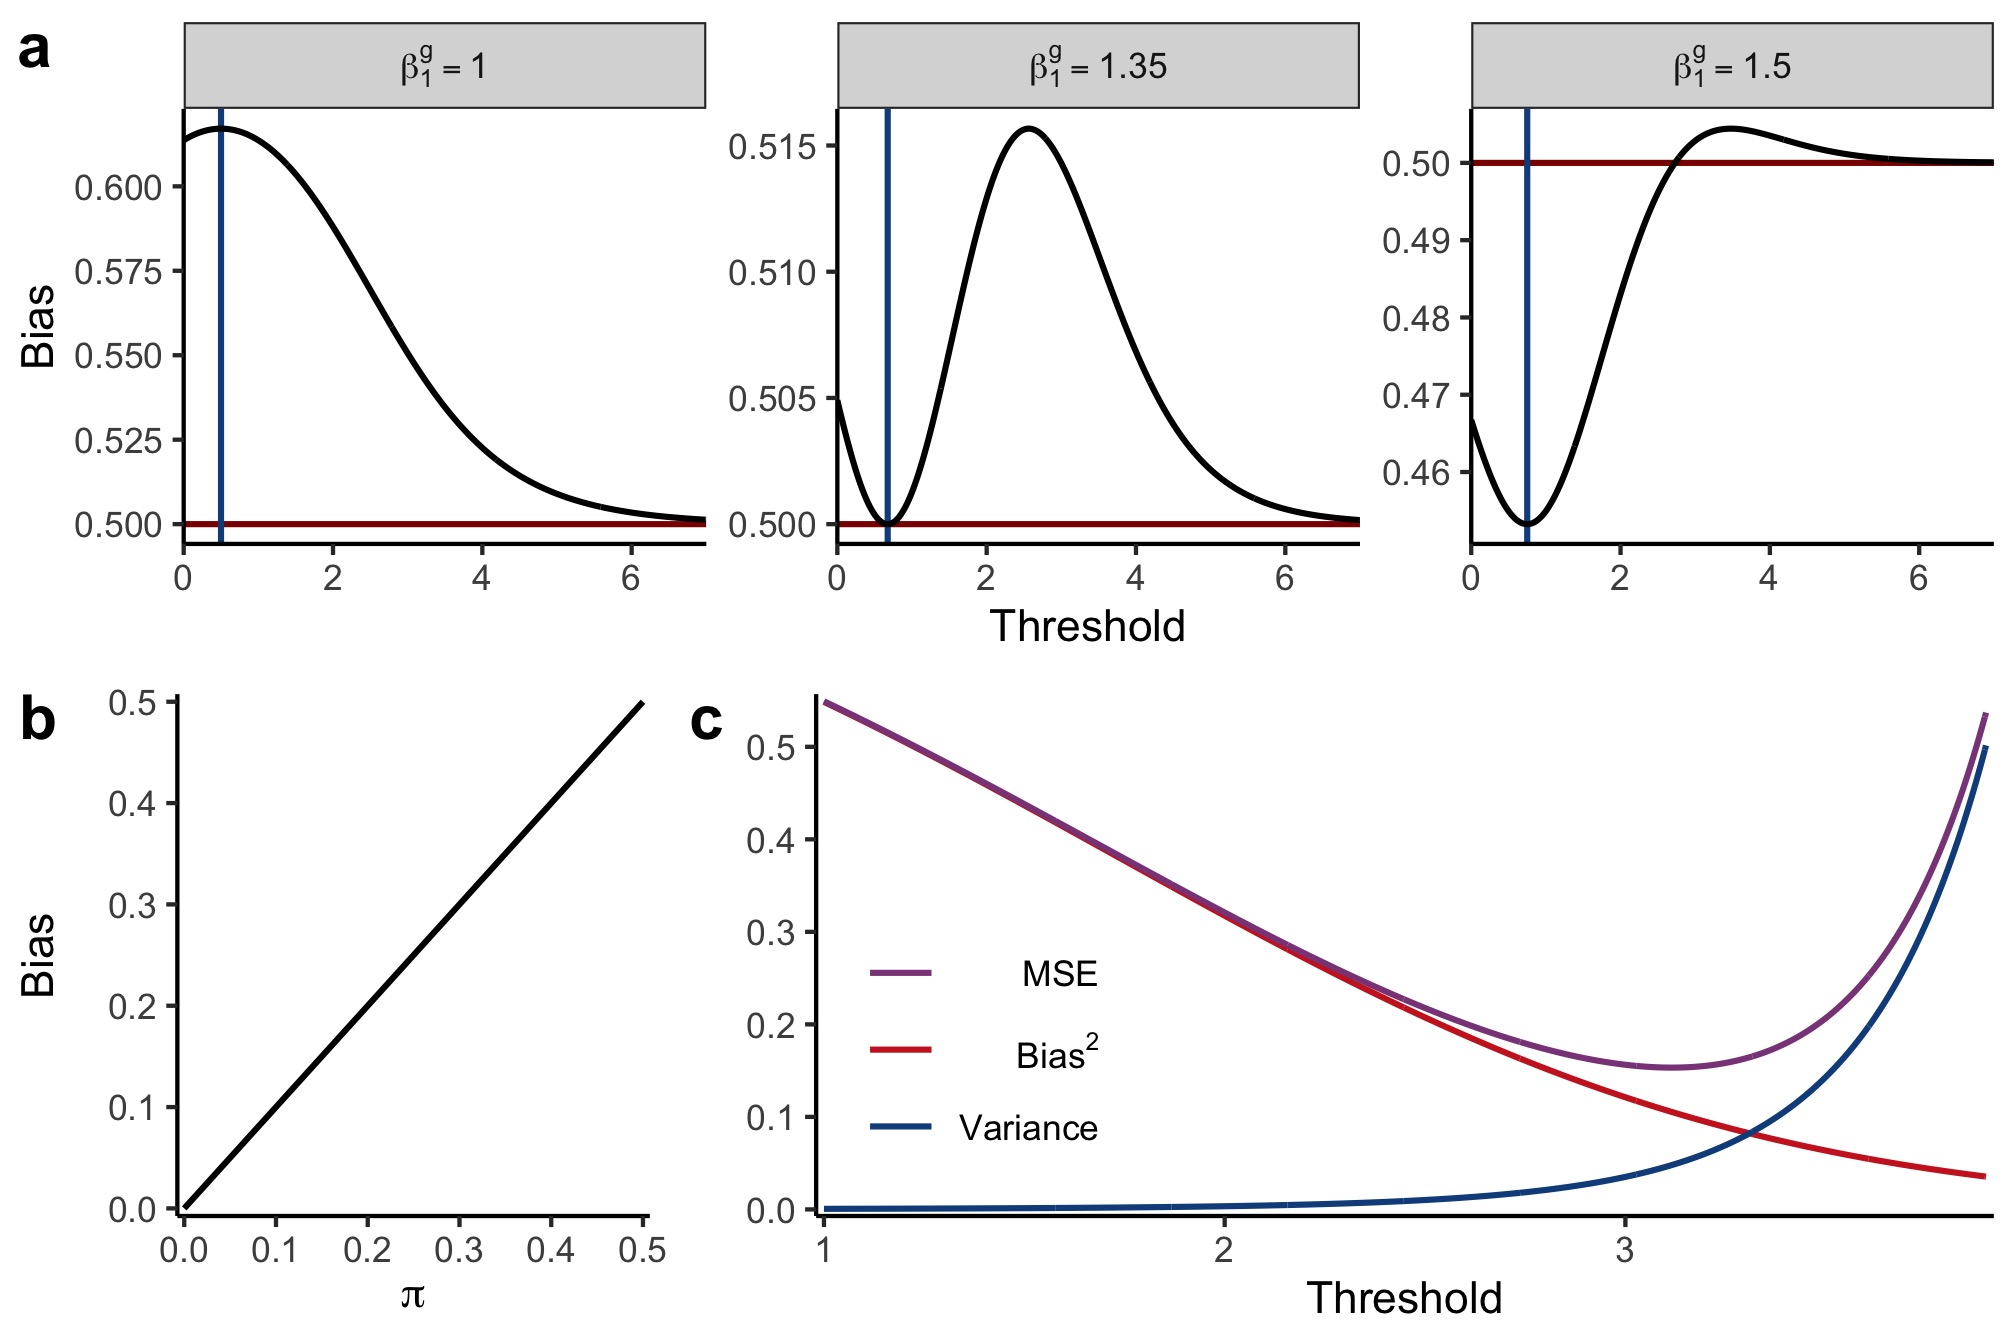
\includegraphics[width=1\linewidth]{../../figures/thresholding_theoretical/plot}
	\caption{\textbf{Theoretical challenges of thresholded regression.} \textbf{a,} Asymptotic relative bias versus threshold for different values of $\beta^g_1$. The bias function is highly nonconvex and strictly nonzero. Vertical blue lines, Bayes-optimal decision boundaries. Across all panels, $\beta^g_0 = 0$ and $\pi = 1/2$. \textbf{b,} Asymptotic relative bias versus $\pi$ when the threshold is set to a large number. The two quantities coincide exactly. \textbf{c,} Bias-variance decomposition for thresholding method in no-intercept model. Bias decreases and variance increases as the threshold tends to infinity. $\beta^g_1 = 1, \beta^m_1 = 1,$ and $\pi = 0.1$.}
	\label{thresholding_theoretical}
\end{figure}

\begin{center}
	\textbf{Bias-variance tradeoff (Panel c)}
\end{center}

Finally, to shed light on limitations of the large threshold selection strategy, we derive an exact bias-variance decomposition for the thresholding estimator. We consider a slightly simpler, no-intercept version of (\ref{theoretical_model}) for this purpose:
\begin{equation}\label{theoretical_model_no_int}
\begin{cases}
m_i = \beta_m p_i + \ep_i \\
g_i = \beta_g p_i + \tau_i \\
p_i \sim \textrm{Bern}(\pi) \\
\ep_i, \tau_i \sim N(0,1) \\
p_i \indep \tau_i \indep \ep_i.
\end{cases}
\end{equation}
The thresholding estimator $\hat{\beta}_m$ in the no-intercept case is
\begin{equation}\label{thresh_estimator_no_int}
 \hat{\beta}_m = \frac{ \sum_{i=1}^n \hat{p}_i m_i }{\sum_{i=1}^n \hat{p}_i^2}. 
\end{equation}
\begin{proposition}\label{prop:bv_decomp}
The limiting distribution of $\hat{\beta}_m$ is
$$\sqrt{n}(\hat{\beta}_m - l) \xrightarrow{d} N\left(0, \frac{ \beta_m\omega\pi(\beta_m - 2l) + \E[\hat{p}_i](1 + l^2) }{\left(\E[\hat{p}_i]\right)^2} \right),$$ where
$$\begin{cases}
l = \beta_m\omega \pi/[\zeta(1-\pi) + \omega \pi], \\
\E[\hat{p}_i] = \pi \omega + (1-\pi) \zeta, \\
\omega = \Phi(\beta_g - c), \\
\zeta = \Phi(- c).\\
\end{cases}
$$
\end{proposition}
This result yields an exact bias-variance decomposition for $\hat{\beta}_m$ for large $n$ (Figure \ref{thresholding_theoretical}c). As the threshold tends to infinity, the bias decreases and the variance increases, consistent with the intuition that a large threshold reduces the misclassification rate at the cost of decreasing the ``effective sample size.'' The best strategy for maximizing estimation accuracy (as quantified by mean squared error) is to select a threshold that induces moderate bias. A downside of this approach, however, is that constructing valid confidence intervals becomes more challenging.

% These difficulties motivate our core research question: does bypassing thresholding altogether lead to better estimation and inference in single-cell CRISPR screens? To answer this question, we propose GLM-EIV, method for single-cell CRISPR screen analysis that models gRNA counts directly.

\section{GLM-EIV}

\section{Simulation studies}

\section{Real data analysis}

\section{Discussion}

\section{Appendix}

\subsection{Theoretical details for thresholding estimator}
This section contains proofs of the propositions presented Section \ref{sec:thresholding_theory}, ``Theoretical analysis of thresholding estimator.'' The subsections are organized as follows. Section (\ref{sec:notation}) introduces some notation. Section (\ref{sec:convergence}) establishes almost sure convergence of the thresholding estimator in the model (\ref{theoretical_model}), proving Proposition \ref{prop:convergence}. Section (\ref{sec:simplication}) simplifies the expression for the attenuation function $\gamma$, and section (\ref{sec:derivatives})  computes derivatives of $\gamma$ to be used throughout the proofs. Section (\ref{sec:c_limit}) establishes the limit in $c$ of $\gamma$, proving Proposition \ref{prop:c_limit} and as a corollary Proposition \ref{prop:c_limit_half}. Section (\ref{sec:bayes_opt}) establishes that the Bayes-optimal decision boundary is a critical value of $\gamma$, proving Proposition \ref{prop:bayes_opt}, and section (\ref{sec:comparison}) compares the competing threshold selection strategies head-to-head, proving Proposition \ref{prop:comparison}. Section (\ref{sec:monotone}) demonstrates that $\gamma$ is monotone in $\beta^g_1$, proving Proposition \ref{prop:monotonic}, and Section (\ref{sec:att_bias}) establishes attenuation bias of the thresholding estimator, proving Proposition \ref{prop:att_bias}. Finally, Section (\ref{sec:bv_decomp}) derives the bias-variance decomposition of the thresholding estimator in the model (\ref{theoretical_model_no_int}), proving Proposition \ref{prop:bv_decomp}.

% Labels of propositions and theorems
% propositions:
% prop:convergence
% prop:att_bias
% prop:bayes_opt
% prop:c_limit_half
% prop:comparison
% prop:monotonic
% prop:c_limit
% prop:bv_decomp

% sections
% sec:notation
% sec:convergence
% sec:simplication
% sec:derivatives
% sec:c_limit
% sec:bayes_opt
% sec:comparison
% sec:beta_lim
% sec:monotone
% sec:att_bias
% sec:bv_decomp

\subsubsection{Notation}\label{sec:notation}
 All notation introduced in this subsection (i.e., \ref{sec:notation}) pertains to the Gaussian model with intercepts (\ref{theoretical_model}). Recall that the attenuation function $\gamma: \R^4 \to \R$ is defined by
$$ \gamma(\beta^g_1, c, \pi, \beta^g_0) = \frac{\pi(\omega - \E[\hat{p}_i])}{ \E[\hat{p}_i](1 -\E[\hat{p}_i])},$$ where $$\begin{cases} \E[\hat{p}_i] = \zeta(1-\pi) + \omega\pi, \\
\omega = \Phi\left(\beta_1^g + \beta_0^g - c \right) ,\\ \zeta = \Phi\left( \beta^g_0 - c \right).
\end{cases}$$ Additionally, recall that the asymptotic relative bias function $b: \R^4 \to \R$ is
$$ b(\beta^g_1, c, \pi, \beta^g_0) = 1 - \gamma(\beta^g_1, c, \pi, \beta^g_0).$$ Next, we define the functions $g$ and $h: \R^4 \to \R$ by
\begin{equation}\label{def_g}
g(\beta^g_1, c, \pi, \beta^g_0) = (1-\pi)\left( \Phi(\beta_0^g + \beta_1^g - c)\right) - (1-\pi)\left(\Phi(\beta_0^g - c)\right)\end{equation}
 and
\begin{multline}\label{def_h}
h(\beta^g_1, c, \pi, \beta^g_0) = \left[(1-\pi)\left( \Phi(\beta_0^g - c)\right) + \pi\left(\Phi(\beta^g_0 + \beta^g_1 - c) \right) \right] \cdot \\ \left[(1-\pi)\left( \Phi(c - \beta^g_0) \right) + \pi\left(\Phi(c - \beta_0^g - \beta_1^g) \right) \right].
\end{multline}
We use $f:\R \to \R$ to denote the $N(0,1)$ density, and we denote the right-tail probability probability of $f$ by $\bar{\Phi}$, i.e., 
$$\bar{\Phi}(x) = \int_{x}^{\infty} f = \Phi(-x).$$

The parameter $\beta^g_0$ is a given, fixed constant throughout the proofs. Therefore, to minimize notation, we typically use $\gamma(\beta^g_1, c, \pi)$ (resp., $b(\beta^g_1, c, \pi),$ $g(\beta^g_1, c, \pi),$ $h(\beta^g_1, c, \pi)$) to refer to the function $\gamma$ (resp., $b, g, h$) evaluated at $(\beta^g_1, c, \pi, \beta^g_0)$. Finally, for a given function $r: \R^{p} \to \R$, point $x \in \R^p$, and index $i \in \{1, \dots, p\}$, we use the symbol $D_i r(x)$ to refer to the derivative of the $i$th component of $r$ evaluated at $x$ (\textit{sensu} \cite{fitzpatrick2009}). For example, $D_1 \gamma(\beta^g_1, c, 1/2)$ is the derivative of the first component of $\gamma$ (the component corresponding to $\beta^g_1$) evaluated at $(\beta^g_1, c, 1/2)$. Likewise,  $D_2g(\beta^g_1, c, \pi)$ is the derivative of the second component of $g$ (the component corresponding to $c$) evaluated at $(\beta^g_1, c, \pi).$

\subsubsection{Almost sure limit of $\hat{\beta}^m_1$}\label{sec:convergence}

We derive the limit in probability of $\hat{\beta}^m_1$ for the Gaussian model with intercepts (\ref{theoretical_model}). Dividing by $n$ in (\ref{thresh_est_intercepts}), we can express $\hat{\beta}^m_1$ as
$$ \hat{\beta}^m_1 = \frac{ \frac{1}{n} \sum_{i=1}^n ( \hat{p}_i - \overline{\hat{p}_i})(m_i - \overline{m})}{ \frac{1}{n} \sum_{i=1}^n (\hat{p}_i - \overline{\hat{p}})}.$$ By weak LLN,
$$ \hat{\beta}^m_1 \xrightarrow{P} \frac{\textrm{Cov}(\hat{p}_i, m_i)}{\V\left(\hat{p}_i\right)}.$$ To compute this quantity, we first compute several simpler quantities:
\begin{itemize}
\item[1.] Expectation of $m_i$: $\E[m_i] = \beta^m_0 + \beta^m_1\pi.$
\item[2.] Expectation of $\hat{p}_i$: \begin{multline*}
\E[\hat{p}_i] = \P\left[\hat{p}_i = 1\right] = \P\left[\beta^g_0 + \beta^g_1 p_i + \tau_i \geq c \right] = \\ \textrm{(By LOTP) } \P\left[ \beta^g_0 + \tau_i \geq c \right]\P\left[p_i = 0\right] + \P\left[ \beta^g_0 + \beta^g_1 + \tau_i \geq c \right] \P[p_i = 1] \\ = \P\left[ \tau_i \geq c - \beta^g_0\right](1- \pi) + \P\left[ \tau_i \geq c - \beta^g_1 - \beta^g_0 \right](\pi) \\ =  \left(\bar{\Phi}(c - \beta^g_0) \right) (1 - \pi) + \left( \bar{\Phi}(c - \beta^g_1 - \beta^g_0) \right)(\pi) = \\  \Phi(\beta^g_0 - c) (1-\pi) + \Phi(\beta^g_1 + \beta^g_0 - c) \pi = \zeta(1-\pi) + \omega \pi.
\end{multline*}
\item[3.] Expectation of $\hat{p}_i p_i$: 
$$\E\left[ \hat{p}_i p_i \right] = \E\left[\hat{p}_i | p_i = 1 \right] \P\left[ p_i =1 \right] = \P\left[ \beta^g_0 + \beta^g_1 + \tau_i \geq c \right] \pi = \omega \pi.$$
\item[4.] Expectation of $\hat{p}_i m_i$:
\begin{multline*}
\E\left[\hat{p}_i m_i\right] = \E[\hat{p}_i (\beta^m_0 + \beta^m_1 p_i + \ep_i)] = \beta^m_0 \E\left[\hat{p}_i\right] + \beta^m_1 \E\left[\hat{p}_i p_i\right] + \E[\hat{p}_i \ep_i] \\ = \beta^m_0 \E[\hat{p}_i] + \beta^m_1 \omega \pi + \E[\hat{p}_i] \E[\ep_i] = \beta^m_0 \E[\hat{p}_i] + \beta^m_1 \omega \pi.
\end{multline*}
\item[5.] Variance of $\hat{p}_i$: Because $\hat{p}_i$ is binary, we have that $\V[\hat{p}_i] = \E[\hat{p}_i]\left(1 - \E[\hat{p}_i]\right) .$
\item[6.] Covariance of $\hat{p}_i, m_i$:
\begin{multline*}
\textrm{Cov}\left(\hat{p}_i, m_i\right) = \E\left[\hat{p}_i m_i\right] - \E[\hat{p}_i] \E[m_i] = \beta^m_0 \E[\hat{p}_i] + \beta^m_1 \omega \pi - \E[\hat{p}_i]( \beta^m_0 + \beta^m_1 \pi)\\ = \beta^m_1 \omega \pi - \E[\hat{p}_i] \beta_1^m \pi = \beta^m_1 \pi \left( \omega - \E[\hat{p}_i]\right).
\end{multline*}
Combining these expressions, we have that
$$ \hat{\beta}^m_1 \xrightarrow{P} \frac{\beta^m_1 \pi (\omega - \E[\hat{p}_i])}{\E[\hat{p}_i](1 - \E[\hat{p}_i])} = \beta^m_1 \gamma(\beta^g_1, c, \pi).$$
\end{itemize}

\subsubsection{Re-expressing $\gamma$ in a simpler form}\label{sec:simplication}
We rewrite the attenuation fraction $\gamma$ in a way that makes it more amenable to theoretical analysis. We leverage the fact that $f$ integrates to unity and is even. We have that
\begin{multline}\label{thm:gamma_expression_1} \E\left[\hat{p}_i\right] = (1 - \pi) \bar{\Phi}(c - \beta_0^g) + \pi \bar{\Phi}(c - \beta^g_0 - \beta^g_1) \\ = (1 - \pi) \Phi(\beta_0^g - c) + \pi\Phi(\beta^g_0 + \beta^g_1 - c), \end{multline}
 and so \begin{multline}\label{thm:gamma_expression_2} 1 - \E\left[\hat{p}_i\right] = (1 - \pi) + \pi - \E[\hat{p}_i]  = (1-\pi) \left(1 - \bar{\Phi}(c - \beta_0^g)\right)  + \pi \left(1 - \bar{\Phi}(c - \beta^g_0 - \beta^g_1) \right) \\ = (1 - \pi)\Phi(c - \beta^g_0) + \pi \Phi(c - \beta_0^g - \beta_1^g).
\end{multline}
Next,
\begin{equation}\label{thm:gamma_expression_3}
\omega = \Phi(\beta^g_1 + \beta^g_0 - c),\end{equation} and so
\begin{multline}\label{thm:gamma_expression_4}
\omega - \E[\hat{p}_i] = \Phi(\beta^g_1 + \beta^g_0 - c) - (1-\pi)\Phi(\beta^g_0 - c) - \pi \Phi(\beta^g_0 + \beta^g_1 - c)  \\ (1-\pi)\Phi(\beta^g_1 + \beta^g_0 - c)  - (1-\pi)\Phi(\beta^g_0 - c).
\end{multline}

Combining (\ref{thm:gamma_expression_1}, \ref{thm:gamma_expression_2}, \ref{thm:gamma_expression_3}, \ref{thm:gamma_expression_4}), we find that
\begin{multline}\label{gamma_alternative}
\gamma(\beta^g_1, c, \pi) = \frac{\pi(\omega - \E[\hat{p}_i])}{\E[\hat{p}_i](1 - \E[\hat{p}_i])} \\ = \frac{\pi \left[(1 - \pi) \Phi(\beta_0^g + \beta_1^g - c) - (1 - \pi) \Phi(\beta_0^g - c)\right]}{\left[(1-\pi)\Phi(\beta_0^g - c) + \pi \Phi(\beta^g_0 + \beta^g_1 - c) \right] \left[(1 - \pi) \Phi(c - \beta^g_0) + \pi\Phi(c - \beta_0^g - \beta_1^g) \right]}.
\end{multline}
As a corollary, when $\pi = 1/2$,
\begin{multline}\label{gamma_alternative_pi_half}
\gamma(\beta^g_1, c, 1/2)  \\ = \frac{\Phi(\beta_0^g + \beta_1^g - c) - \Phi(\beta_0^g - c) }{\left[\Phi(\beta_0^g - c) +\Phi(\beta^g_0 + \beta^g_1 - c)\right] \left[\Phi(c - \beta^g_0) + \Phi(c - \beta_0^g - \beta_1^g) \right]}.
\end{multline}
Recalling the definitions of $g$ (\ref{def_g}) and $h$ (\ref{def_h}), we can write $\gamma$ as
$$ \gamma(\beta^g_1, c, \pi) = \frac{\pi g(\beta^g_1, c, \pi)}{h(\beta^g_1, c,\pi)}.$$
The special case (\ref{gamma_alternative_pi_half}) is identical to
\begin{equation}\label{gamma_alt2_pi_half}
\gamma(\beta^g_1, c, 1/2) = \frac{(4)(1/2)g(\beta^g_1, c, 1/2)}{4 h(\beta^g_1, c, 1/2)} = \frac{2 g(\beta^g_1, c, 1/2)}{4h(\beta^g_1, c, 1/2)},
\end{equation}
i.e., the numerator and denominator of  (\ref{gamma_alt2_pi_half}) coincide with those of (\ref{gamma_alternative_pi_half}). We sometimes will use the notation $2\cdot g$ and $4\cdot h$ to refer to the numerator and denominator of (\ref{gamma_alternative_pi_half}), respectively.

\subsubsection{Derivatives of  $g$ and $h$ in $c$}\label{sec:derivatives}
We compute the derivatives of $g$ and $h$ in $c$, which we will need to prove subsequent results. First, by FTC and the evenness of $f$, we have that
\begin{multline}\label{dg_dc}
D_2 g(\beta^g_1, c, \pi) = -(1-\pi)f( \beta^g_0 + \beta^g_1 - c ) + (1-\pi) f(\beta^g_0 - c) \\ = (1-\pi) f(c - \beta^g_0) - (1-\pi)f(c - \beta^g_0 - \beta^g_1).
\end{multline}
Second, we have that
\begin{multline}\label{dh_dc}
D_2 h(\beta^g_1, c, \pi) \\ = -[(1-\pi)f(\beta^g_0 - c) + \pi f( \beta^g_0 + \beta^g_1 - c )]\left[(1-\pi)\Phi(c - \beta^g_0) + \pi \Phi(c - \beta_0^g - \beta_1^g)  \right] \\ + [(1-\pi) f(c - \beta^g_0) +  \pi f(c - \beta^g_0 - \beta^g_1)] \left[(1-\pi) \Phi(\beta_0^g - c) + \pi \Phi(\beta^g_0 + \beta^g_1 - c) \right] \\ = \left[ (1-\pi) f(c - \beta^g_0) +  \pi f(c - \beta^g_0 - \beta^g_1) \right] \cdot \\ \bigg[ (1-\pi) \Phi(\beta_0^g - c) + \pi\Phi(\beta^g_0 + \beta^g_1 - c) \\ - (1-\pi) \Phi(c - \beta^g_0) - \pi \Phi(c - \beta_0^g - \beta_1^g) \bigg].
\end{multline}

\subsubsection{Limit of $\gamma$ in $c$}\label{sec:c_limit}

Assume (without loss of generality) that $\beta^g_1 > 0$. We compute $\lim_{c \to \infty} \gamma(\beta^g_1, c, \pi)$. Observe that $$\lim_{c \to \infty} g(\beta^g_1, c, \pi) = \lim_{c \to \infty} h(\beta^g_1, c, \pi)  = 0.$$ Therefore, we can apply L'H\^{o}pital's rule. We have by (\ref{dg_dc}) and (\ref{dh_dc}) that \begin{multline}\label{c_limit_product}
\lim_{c \to \infty} \gamma(\beta^g_1, c, \pi) = \lim_{c \to \infty} \frac{\pi D_2 g(\beta^g_1, c, \pi)}{D_2h(\beta^g_1, c, \pi)} \\ = \lim_{c \to \infty} \bigg\{ \frac{(1-\pi) f(c - \beta^g_0) + \pi f(c - \beta^g_0 - \beta^g_1)}{\pi (1-\pi) f(c - \beta^g_0) - \pi (1-\pi)f(c - \beta^g_0 - \beta^g_1)} \\ \cdot \bigg[ (1-\pi) \Phi(\beta_0^g - c) + \pi \Phi(\beta^g_0 + \beta^g_1 - c) \\ - (1-\pi) \Phi(c - \beta^g_0) - \pi \Phi(c - \beta_0^g - \beta_1^g) \bigg] \bigg\}^{-1}.
 \end{multline}
 We evaluate the two terms in the product (\ref{c_limit_product}) separately. Dividing by $f(c - \beta^g_0 - \beta^g_1) > 0$, we see that
 \begin{equation}\label{c_limit_product_2}
 \frac{(1-\pi) f(c - \beta^g_0) + \pi f(c - \beta^g_0 - \beta^g_1)}{\pi (1-\pi) f(c - \beta^g_0) - \pi (1-\pi)f(c - \beta^g_0 - \beta^g_1)} = \frac{\frac{(1-\pi) f(c - \beta^g_0)}{ f(c - \beta^g_0 - \beta^g_1)} + \pi}{\frac{ \pi(1-\pi) f(c - \beta^g_0)}{ f(c - \beta^g_0 - \beta^g_1)} - \pi(1-\pi)}.
 \end{equation}
 To evaluate the limit of (\ref{c_limit_product_2}), we first evaluate the limit of
 \begin{multline}\label{c_limit_product_3}
 \frac{f(c - \beta^g_0)}{f(c - \beta^g_0 - \beta^g_1)} = \frac{\exp{[-(1/2)(c - \beta_0^g)^2]}}{\exp{[-(1/2)( c - \beta^g_0 - \beta^g_1)^2]}} \\ = \frac{\exp[ -(1/2)(c^2 - 2 c \beta^g_0 + (\beta^g_0)^2)]}{\exp\left[-(1/2)( c^2 - 2c \beta^g_0 - 2 c \beta^g_1 + (\beta^g_0)^2 + 2( \beta^g_0 \beta^g_1) + (\beta^g_1)^2)\right]} \\ = \exp\big[-c^2/2 + c \beta^g_0 - (\beta^g_0)^2/2 \\ + c^2/2 - c \beta^g_0 - c \beta^g_1 + (\beta^g_0)^2/2 + \beta^g_0 \beta^g_1 + (\beta^g_1)^2/2 \big] \\ = \exp[ -c \beta^g_1 + \beta^g_0 \beta^g_1 + (\beta^g_1)^2/2] = \exp[ \beta^g_0 \beta^g_1 + (\beta^g_1)^2/2]\exp[ -c \beta^g_1]. 
\end{multline}
Taking the limit in (\ref{c_limit_product_3}), we obtain
$$
\lim_{c \to \infty} \frac{f(c - \beta^g_0)}{f(c - \beta^g_0 - \beta^g_1)} = \exp[ \beta^g_0 \beta^g_1 + (\beta^g_1)^2/2] \lim_{c \to \infty} \exp[ -c \beta^g_1] = 0
$$ for $\beta^g_1 > 0$. We now can evaluate the limit of (\ref{c_limit_product_2}):
$$ \lim_{c \to \infty} \frac{(1-\pi) f(c - \beta^g_0) + \pi f(c - \beta^g_0 - \beta^g_1)}{\pi (1-\pi) f(c - \beta^g_0) - \pi (1-\pi)f(c - \beta^g_0 - \beta^g_1)} = \frac{-\pi}{\pi(1-\pi)} = -\frac{1}{1 -\pi}.$$ Next, we compute the limit of the other term in the product (\ref{c_limit_product}):
\begin{multline}\label{c_limit_product_4}
\lim_{c \to \infty} \bigg[ (1-\pi)\Phi(\beta_0^g - c) + \pi \Phi(\beta^g_0 + \beta^g_1 - c) \\ - (1-\pi)\Phi(c - \beta^g_0) - \pi \Phi(c - \beta_0^g - \beta_1^g) \bigg] = -(1-\pi) - \pi = -1.
\end{multline}
Combining (\ref{c_limit_product_2}) and (\ref{c_limit_product_4}), the limit (\ref{c_limit_product}) evaluates to
$$ \lim_{c \to \infty} \gamma(\beta^g_1, c, \pi) = \left(  \frac{ 1 }{ 1 - \pi }\right)^{-1} = 1 - \pi.$$ It follows that the limit in $c$ of the asymptotic relative bias $b$ is
$$\lim_{c \to \infty} b(\beta^g_1, c, \pi) = 1 - \lim_{c \to \infty} \gamma(\beta^g_1, c, \pi) = \pi.$$
A corollary is that
$$\lim_{c \to \infty} b(\beta^g_1, c, 1/2) = 1/2.$$

\subsubsection{Bayes-optimal decision boundary as a critical value of $\gamma$}\label{sec:bayes_opt}
Let $c_\textrm{bayes} = \beta^g_0 + (1/2)\beta^g_1.$ We show that $c = c_\textrm{bayes}$ is a critical value of $\gamma$ for $\pi = 1/2$ and given $\beta^g_1$, i.e, $$D_2 \gamma (\beta^g_1, c_\textrm{bayes}, 1/2) = 0.$$ Differentiating (\ref{gamma_alt2_pi_half}), the quotient rule implies that
\begin{equation}\label{quotient_rule}
D_2\gamma(\beta^g_1, c, 1/2) \\ = \frac{D_2[2g(\beta^g_1, c, 1/2)] 4h(\beta^g_1, c, 1/2) - 2g(\beta^g_1, c, 1/2) D_2[4h(\beta^g_1, c, 1/2)]}{[4h(\beta^g_1, c, \pi)]^2}.
\end{equation}
We have by (\ref{dg_dc}) that
\begin{equation}\label{dg_dc_bayes}
D_2[2g(\beta^g_1, c_\textrm{bayes}, 1/2)] = f( \beta^g_1/2) - f( -\beta^g_1/2) = f(\beta^g_1/2) - f(\beta^g_1/2) = 0.
\end{equation}
Similarly, we have by (\ref{dh_dc}) that
\begin{multline}\label{dh_dc_bayes}
D_2[4 h(\beta^g_1, c_\textrm{bayes}, \pi)] = [f( \beta^g_1/2) + f( -\beta^g_1/2)] \cdot \\ \left[  \Phi(-\beta^g_1/2) + \Phi(\beta^g_1/2) -  \Phi(\beta^g_1/2) - \Phi(-\beta^g_1/2) \right] = 0.
\end{multline}
Plugging in (\ref{dh_dc_bayes}) and (\ref{dg_dc_bayes}) to (\ref{quotient_rule}), we find that 
$$D_2[\gamma(\beta^g_1, c_\textrm{bayes}, 1/2)] = 0.$$ Finally, because
$$b(\beta^g_1, c, 1/2) = 1 - \gamma(\beta^g_1, c, 1/2),$$ it follows that
$$D_2[b(\beta^g_1, c_\textrm{bayes}, 1/2)] = -D_2[\gamma(\beta^g_1, c_\textrm{bayes}, 1/2)] = 0.$$

\subsubsection{Comparing Bayes-optimal decision boundary and large threshold}\label{sec:comparison}

We compare the bias produced by setting the threshold to a large number to the bias produced by setting the threshold to the Bayes-optimal decision boundary. Let $r: \R^{\geq 0} \to \R$ be the value of attenuation function evaluated at the Bayes-optimal decision boundary $c_\textrm{bayes} = \beta^g_0 + (1/2) \beta^g_1$, i.e.
\begin{multline*}
r(\beta^g_1) = \gamma(\beta^g_1, \beta^g_0 + (1/2)\beta^g_1, 1/2) = \frac{\Phi(\beta^g_1/2) - \Phi(-\beta^g_1/2)}{\left[\Phi(-\beta^g_1/2) + \Phi( \beta^g_1/2) \right] \left[\Phi(\beta^g_1/2) + \Phi( -\beta^g_1/2)\right]} \\ = \frac{\int_{-\beta^g_1/2}^{\beta^g_1/2} f}{\left[ 1 - \Phi(\beta^g_1/2) + \Phi(\beta^g_1/2) \right]\left[ \Phi(\beta^g_1/2) + 1 - \Phi(\beta^g_1/2) \right]} = 2 \int_{0}^{\beta^g_1/2} f = 2 \Phi(\beta^g_1/2) - 1.
\end{multline*}
We set $r$ to $1/2$ and solve for $\beta^g_1$:
\begin{multline*}
r(\beta^g_1) = 1/2 \iff 2\Phi(\beta^g_1/2) -1 = 1/2 \\ \iff \Phi(\beta^g_1/2) = 3/4 \iff \beta^g_1 = 2 \Phi^{-1}(3/4) \approx 1.35.
\end{multline*}
Because $r$ is a strictly increasing function, it follows that $r(\beta^g_1) < 1/2$ for $\beta^g_1 < 2\Phi^{-1}(3/4)$ and $r(\beta^g_1) > 1/2$ for $\beta^g_1 > 2\Phi^{-1}(3/4).$ Next, because $$b(\beta^g_1, c_\textrm{bayes}, 1/2) = 1 - \gamma(\beta^g_1, c_\textrm{bayes}, 1/2) = 1 - r(\beta^g_1),$$ we have that $b(\beta^g_1, c_\textrm{bayes}, 1/2) > 1/2$ for $\beta^g_1 < 2 \Phi^{-1}(3/4)$ and $b(\beta^g_1, c_\textrm{bayes}, 1/2) < 1/2$ for $\beta^g_1 > 2 \Phi^{-1}(3/4)$. Recall that the bias induced by sending the threshold to infinity (as stated in Proposition \ref{prop:c_limit_half} and proven in Section \ref{sec:c_limit}) is $1/2$, i.e. $$b(\beta^g_1, \infty, 1/2) = 1/2.$$ We conclude that $b(\beta^g_1, c_\textrm{bayes},1/2) > b(\beta^g_1, \infty, 1/2)$ on $\beta^g_1 \in [0, 2\Phi^{-1}(3/4))$; $b(\beta^g_1, c_\textrm{bayes},1/2) = b(\beta^g_1, \infty, 1/2)$ for $\beta^g_1 = 2\Phi^{-1}(3/4)$; and $b(\beta^g_1, c_\textrm{bayes},1/2) < b(\beta^g_1, \infty, 1/2)$ on $\beta^g_1 \in (2\Phi^{-1}(3/4), \infty)$.

\subsubsection{Monotonicity in $\beta^g_1$}\label{sec:monotone}
We show that $\gamma$ is monotonically increasing in $\beta^g_1$ for $\pi = 1/2$ and given threshold $c$. We begin by stating and proving two lemmas. The first lemma establishes an inequality that will serve as the basis for the proof.

\begin{lemma}
The following inequality holds: 
\begin{multline}\label{basic_ineq_cp}
\left[\Phi(\beta^g_0 - c) + \Phi(\beta^g_0 + \beta^g_1 - c) \right] \\ \cdot \left[\Phi(\beta_0^g + \beta_1^g - c) - \Phi(\beta_0^g - c) + \Phi(c - \beta^g_0) + \Phi(c - \beta_0^g - \beta_1^g) \right] \\ \geq \left[\Phi(\beta_0^g + \beta_1^g - c) - \Phi(\beta_0^g - c)\right]\left[\Phi(c - \beta^g_0) + \Phi(c - \beta_0^g - \beta_1^g)\right].
\end{multline}
\end{lemma}
\textbf{Proof}: We take cases on the sign on $\beta^g_1$.

\noindent
\underline{Case 1}: $\beta^1_g < 0$. Then $ \beta^g_1 + (\beta^g - c) < (\beta^g_0 - c),$ implying $\Phi(\beta^g_0 + \beta^g_1 - c) < \Phi(\beta^g_0 - c),$ or $[\Phi(\beta^g_0 + \beta^g_1 - c) - \Phi(\beta^g_0 - c)] < 0.$ Moreover, $[\Phi(c - \beta^g_0) + \Phi(c - \beta_0^g - \beta_1^g)]$ is positive. Therefore, the right-hand side of (\ref{basic_ineq_cp}) is negative.

Turning our attention of the left-hand side of (\ref{basic_ineq_cp}), we see that
\begin{equation}\label{basic_ineq_cp_2}
\Phi(\beta^g_0 + \beta^g_1 - c) + \Phi( c - \beta^g_0 - \beta^g_1) = 1 -\Phi(\beta^g_0 + \beta^g_1 - c) + \Phi( c - \beta^g_0 - \beta^g_1) = 1.
\end{equation}
Additionally, $\Phi(\beta^g_0 - c) < 1$ and $ \Phi(c - \beta^g_0) > 0$. Combining these facts with (\ref{basic_ineq_cp_2}), we find that
$$ \left[\Phi(\beta_0^g + \beta_1^g - c) - \Phi(\beta_0^g - c) + \Phi(c - \beta^g_0) + \Phi(c - \beta_0^g - \beta_1^g) \right] > 0. $$ Finally, because $\left[\Phi(\beta^g_0 - c) + \Phi(\beta^g_0 + \beta^g_1 - c) \right] > 0,$ the entire left-hand side of (\ref{basic_ineq_cp}) is positive. The inequality holds for $\beta^g_1 < 0$.

\noindent
\underline{Case 2}: $\beta^1_g \geq 0.$  We will show that the first term on the LHS of (\ref{basic_ineq_cp}) is greater than the first term on the RHS of (\ref{basic_ineq_cp}), and likewise that the second term on the LHS is greater than the second term on the RHS, implying the truth of the inequality. Focusing on the first term, the positivity of $\Phi(\beta^g_0 -c)$ implies that
$$ \Phi(\beta^g_0 - c) \geq - \Phi(\beta^g_0 - c),$$ and so
$$ \Phi(\beta^g_0 - c) + \Phi(\beta^g_0 + \beta^g_1 - c) \geq \Phi(\beta^g_0 - \beta^g_1 - c) - \Phi(\beta^g_0 - c).$$
Next, focusing on the second term, $\beta^g_1 \geq 0$ implies that 
\begin{equation}\label{basic_ineq_cp_3}
\beta^g_1 + \beta^g_0 - c \geq \beta^g_0 - c \implies \Phi(\beta^g_1 + \beta^g_0 - c) - \Phi(\beta^g_0 - c) \geq 0.
\end{equation}
Adding $\Phi(c - \beta^g_0) + \Phi(c - \beta^g_0 - \beta^g_1)$ to both sides of (\ref{basic_ineq_cp_3}) yields
\begin{multline*}
\Phi(\beta^g_1 + \beta^g_0 - c) - \Phi(\beta^g_0 - c) + \Phi(c - \beta^g_0) + \Phi(c - \beta^g_0 - \beta^g_1) \\ \geq \Phi(c - \beta^g_0) + \Phi(c - \beta^g_0 - \beta^g_1). \textrm{ }
\end{multline*}
The inequality holds for $\beta^g_1 \geq 0$. Combining the cases, the inequality holds for all $\beta^g_1 \in \R$. $\square$

The second lemma establishes the derivatives of the functions $2\cdot g$ and $4 \cdot h$ in $\beta^g_1$.
\begin{lemma}
The derivatives in $\beta^g_1$ of $2\cdot g$ and $4\cdot h$ are
\begin{equation}\label{dg_dbeta}
\textcolor{violet}{D_1[2g(\beta^g_1, c, 1/2)] = f(\beta^g_0 + \beta^g_1 - c)}
\end{equation}
and
\begin{multline}\label{dh_dbeta}
\textcolor{teal}{D_1[4h(\beta^g_1, c, 1/2)] = f(\beta^g_0 + \beta^g_1 - c) \left[\Phi(c - \beta^g_0) + \Phi(c - \beta_0^g - \beta_1^g) \right]} \\ \textcolor{teal}{- f(\beta^g_0 + \beta^g_1 - c) \left[\Phi(\beta_0^g - c) + \Phi(\beta^g_0 + \beta^g_1 - c) \right]}.\end{multline}
\end{lemma}
\textbf{Proof}: Apply FTC and product rule. $\square$

We are ready to prove the monotonicity of $\gamma$ in $\beta^g_1$. Subtracting $$\left[\Phi(\beta_0^g - c) + \Phi(\beta^g_0 + \beta^g_1 - c) \right]\left[\Phi(\beta_0^g + \beta_1^g - c) - \Phi(\beta_0^g - c)\right]$$ from both sides of (\ref{basic_ineq_cp}) and multiplying by $f(\beta^g_0 + \beta^g_1 - c) > 0$ yields
\begin{multline}\label{basic_ineq_cp_4}
\textcolor{violet}{f(\beta^g_0 + \beta^g_1 - c)} \textcolor{red}{ \left[\Phi(\beta^g_0 - c) + \Phi\left(\beta^g_0 + \beta^g_1 - c \right) \right] \left[ \Phi(c - \beta^g_0) + \Phi(c - \beta^g_0 - \beta^g_1) \right]}  \\ \geq \textcolor{teal}{f(\beta^g_0 + \beta^g_1 - c) \left[\Phi(c - \beta^g_0) + \Phi(c - \beta_0^g - \beta_1^g)\right]}\textcolor{blue}{\left[\Phi(\beta_0^g + \beta_1^g - c) - \Phi(\beta_0^g - c)\right]} \\ -\textcolor{teal}{f(\beta^g_0 + \beta^g_1 - c)   \left[\Phi(\beta_0^g - c) + \Phi(\beta^g_0 + \beta^g_1 - c) \right]} \textcolor{blue}{\left[\Phi(\beta_0^g + \beta_1^g - c) - \Phi(\beta_0^g - c)\right]}.
\end{multline}
Next, recall that
\begin{equation}\label{def_2g}
\textcolor{blue}{2g(\beta^g_1,c,1/2) = \Phi(\beta^g_0 + \beta^g_1 - c) - \Phi(\beta^g_0 - c)}.
\end{equation}
and
\begin{equation}\label{def_4h}
\textcolor{red}{4h(\beta^g_1, c, 1/2) = \left[ \Phi(\beta^g_0 - c) + \Phi(\beta^g_0 + \beta^g_1 - c) \right] \left[\Phi(c - \beta^g_0) + \Phi( c - \beta^g_0 - \beta^g_1) \right]}.
\end{equation}
Substituting (\ref{dg_dbeta}, \ref{dh_dbeta}, \ref{def_2g}, \ref{def_4h}) into (\ref{basic_ineq_cp_4}) produces
\begin{equation*}
\textcolor{violet}{D_1[2g(\beta^g_1, c, 1/2)]}\textcolor{red}{4h(\beta^g_1, c, 1/2)} \geq \textcolor{blue}{2g(\beta^g_1, c, 1/2)}\textcolor{teal}{D_1[4h(\beta^g_1, c, 1/2)]},
\end{equation*}
or 
\begin{equation}\label{basic_ineq_cp_5}
\textcolor{violet}{D_1[2g(\beta^g_1, c, 1/2)]}\textcolor{red}{4h(\beta^g_1, c, 1/2)} - \textcolor{blue}{2g(\beta^g_1, c, 1/2)}\textcolor{teal}{D_1[4h(\beta^g_1, c, 1/2)]} \geq 0.
\end{equation}
The quotient rule implies that
\begin{multline}\label{d_gamma_d_beta}
D_1 \gamma(\beta^g_1, c, 1/2) \\ = \frac{ \textcolor{violet}{D_1[2g(\beta^g_1, c, 1/2)]}\textcolor{red}{4h(\beta^g_1, c, 1/2)} - \textcolor{blue}{2g(\beta^g_1, c, 1/2)}\textcolor{teal}{D_1[4h(\beta^g_1, c, 1/2)]} }{[4h(\beta^g_1, c, 1/2)]^2}.
\end{multline}
We conclude by (\ref{basic_ineq_cp_5}) and (\ref{d_gamma_d_beta}) that $\gamma$ is monotonically increasing in $\beta^g_1$. Finally, $b(\beta^g_1, c, \pi) = 1 - \gamma(\beta^g_1, c, \pi)$ is monotonically decreasing in $\beta^g_1$.

\subsubsection{Strict attenuation bias}\label{sec:att_bias}

We begin by computing the limit of $\gamma$ in $\beta^g_1$ given $\pi = 1/2$.  First,
\begin{multline*}
\lim_{\beta^g_1 \to \infty} \gamma(\beta^g_1, c, 1/2) = \frac{1 - \Phi(\beta^g_0 - c)}{\left[1 + \Phi(\beta^g_0 - c) \right] \left[\Phi(c - \beta^g_0) \right]} \\ = \frac{\Phi(c - \beta^g_0)}{ \left[1 + \Phi(\beta^g_0 - c) \right] \left[\Phi(c - \beta^g_0) \right]} = \frac{1}{1 + \Phi(\beta^g_0 - c)} < 1.
\end{multline*}
Similarly,
\begin{multline*}
\lim_{\beta^g_1 \to -\infty} \gamma(\beta^g_1, c, 1/2) = \frac{ - \Phi(\beta^g_0 - c)}{\left[\Phi(\beta^g_0 - c)\right] \left[\Phi(c - \beta^g_0) + 1 \right]} = \frac{-1}{1 + \Phi(c - \beta^g_0)} > -1.
\end{multline*}
The function $\gamma(\beta^g_1, c, 1/2, \beta^g_0)$ is monotonically increasing in $\beta^g_1$ (as stated in Proposition \ref{prop:monotonic} and proven in section \ref{sec:monotone}). It follows that 
$$-1 < -\frac{1}{1 + \Phi(c - \beta^g_0)} \leq \gamma(\beta^g_1, c, 1/2, \beta^g_0) \leq \frac{1}{1 - \Phi(\beta^g_0 - c)} < 1$$ for all $\beta^g_1 \in \R$. But $\beta^g_0$ and $c$ were chosen arbitrarily, and so
$$-1 < \gamma(\beta^g_1, c, 1/2, \beta^g_0) < 1$$ for all $(\beta^g_1, c, \beta^g_0) \in \R^3$. Finally, because $b(\beta^g_1, c, 1/2, \beta^g_0) = 1 - \gamma(\beta^g_1, c, 1/2, \beta^g_0)$, it follows that
$$ 0 < b(\beta^g_1, c, 1/2, \beta^g_0) < 2$$ for all $(\beta^g_1, c, \beta^g_0) \in \R^3$

\subsubsection{Bias-variance decomposition in no-intercept model}\label{sec:bv_decomp}
 
We prove the bias-variance decomposition for the no-intercept model (\ref{theoretical_model_no_int}). Define $l$ (for ``limit'') by
$$l = \beta_m \left(\frac{\omega \pi}{\zeta(1-\pi) + \omega \pi}\right),$$ where
$$
\begin{cases}
\omega = \bar{\Phi}(c - \beta_g) = \Phi(\beta_g - c) \\
\zeta = \bar{\Phi}(c) = \Phi(-c).
\end{cases}
$$
We have that
\begin{equation*}
\hat{\beta}_m - l = \frac{\sum_{i=1}^n \hat{p}_i m_i}{ \sum_{i=1}^n \hat{p}^2_i} - l = \frac{\sum_{i=1}^n \hat{p}_i m_i}{ \sum_{i=1}^n \hat{p}^2_i} - \frac{l \sum_{i=1}^n \hat{p}_i^2 }{ \sum_{i=1}^n \hat{p}_i^2} \\ = \frac{\sum_{i=1}^n \hat{p}_i(m_i - l \hat{p}_i)}{ \sum_{i=1}^n \hat{p}_i^2}.
\end{equation*}
Therefore,
\begin{equation}\label{bc_decomp_1}
\sqrt{n}(\hat{\beta}_m - l) = \frac{(1/\sqrt{n})\sum_{i=1}^n \hat{p}_i(m_i - l \hat{p}_i)}{(1/n)\sum_{i=1}^n \hat{p}_i^2}.
\end{equation}
Next, we compute the expectation and variance of $\hat{p}_i(m_i - l\hat{p}_i)$. To do so, we first compute several simpler quantities:
\begin{enumerate}
\item Expectation of $\hat{p}_i$: 
\begin{multline*}
\E[\hat{p}_i] = \P(p_i\beta_g + \tau_i \geq c) =  \P(\beta_g + \tau_i \geq c)\pi + \P(\tau_i \geq c)(1-\pi) \\ = \pi \omega + (1-\pi)\zeta.
\end{multline*}
\item Expectation of $\hat{p}_i p_i$: $$\E\left[\hat{p}_i p_i\right] = \E\left[\hat{p}_i | p_i = 1 \right]\P\left[p_i = 1\right] = \omega \pi.$$
\item Expectation of $\hat{p}_i m_i$:
\begin{multline*}
\E[\hat{p}_i m_i] = \E\left[\hat{p}_i(\beta_m p_i + \ep_i)\right] = \E\left[\beta_m \hat{p}_i p_i + \hat{p}_i \ep_i \right] \\ = \beta_m \E\left[ \hat{p}_i p_i \right] + \E[\hat{p}_i]\E[\ep_i] = \beta_m \omega \pi + 0 = \beta_m \omega \pi.
\end{multline*}
\item Expectation of $\hat{p}_i m_i^2$: \begin{multline*}
\E\left[\hat{p}_i m_i^2\right] = \E \left[ \hat{p}_i( \beta_m p_i + \ep_i )^2 \right] = \E\left[ \hat{p}_i \left( \beta_m^2 p_i^2 + 2 \beta_m p_i \ep_i + \ep_i^2 \right)  \right] \\ = \E\left[ \hat{p}_i p_i \beta^2_m + 2 \beta_m p_i \hat{p}_i \ep_i + \hat{p}_i \ep_i^2 \right] = \beta^2_m \E[ \hat{p}_i p_i] + 2 \beta_m \E[p_i\hat{p}_i] \E[\ep_i] + \E[\hat{p}_i] \E[ \ep^2_i ] \\ = \beta^2_m \E[ \hat{p}_i p_i] + \E[\hat{p}_i] = \beta^2_m \omega \pi + \E[ \hat{p}_i]. 
\end{multline*}
\end{enumerate}

Now, we can compute the expectation and variance of $\hat{p}_i(m_i - l\hat{p}_i)$. First,
\begin{multline}\label{bv_decomp_2}
\E\left[\hat{p}_i(m_i - l\hat{p}_i) \right] = \E[\hat{p}_i m_i] - l \E[\hat{p}_i] \\ = \beta_m \omega \pi - \left(\frac{\beta_m \omega \pi}{\zeta (1-\pi) + \omega \pi}\right)[\zeta (1-\pi) + \omega \pi] = 0.
\end{multline}
Additionally,
\begin{multline}\label{bv_decomp_3}
\V\left[\hat{p}_i(m_i - l\hat{p}_i)\right] = \E\left[\hat{p}_i^2(m_i - l\hat{p}_i)^2\right] - (\E\left[ \hat{p}_i(m_i - l\hat{p}_i)\right])^2 \\ = \E\left[ \hat{p}_i m_i^2\right] - 2l \E[m_i\hat{p}_i] +l^2 \E[\hat{p}_i]= \beta^2_m \omega \pi + \E[ \hat{p}_i] -2l \beta_m \omega \pi + l^2 \E[\hat{p}_i] \\ = \beta_m\omega\pi(\beta_m - 2l) + \E[\hat{p}_i](1 + l^2).
\end{multline}
Therefore, by CLT, (\ref{bv_decomp_2}), and (\ref{bv_decomp_3}),
\begin{equation}\label{bv_decomp_4}
(1/\sqrt{n})\sum_{i=1}^n \hat{p}_i(m_i - l \hat{p}_i) \xrightarrow{d} N\left(0, \beta_m\omega\pi(\beta_m - 2l) + \E[\hat{p}_i](1 + l^2) \right).
\end{equation}
Next, by weak LLN,
\begin{equation}\label{bv_decomp_5}
(1/n) \sum_{i=1}^n \hat{p}_i^2 = (1/n) \sum_{i=1}^n \hat{p}_i \xrightarrow{P} \E[\hat{p}_i].
\end{equation}
Finally, by (\ref{bc_decomp_1}), (\ref{bv_decomp_4}), (\ref{bv_decomp_5}), and Slutsky's Theorem,
$$ \sqrt{n}(\hat{\beta}_m - l) \xrightarrow{d} N\left(0, \frac{ \beta_m\omega\pi(\beta_m - 2l) + \E[\hat{p}_i](1 + l^2) }{\left(\E[\hat{p}_i]\right)^2} \right).$$ Thus, for large $n \in \N$, we have that 
$$ \begin{cases}
\E [\hat{\beta}_m] \approx l, \\
\V[\hat{\beta}_m] \approx \left[\beta_m\omega\pi(\beta_m - 2l) + \E[\hat{p}_i](1 + l^2)\right]/[n\E^2[\hat{p}_i]],
\end{cases}$$
completing the bias-variance decomposition.

\subsection{Derivation of EM algorithm}

\subsection{Derivation of observed information matrix}

\subsection{Implementation using R family objects}

\subsection{Statistical accelerations to GLM-EIV}

\subsection{Additional simulation results}


\bibliographystyle{unsrt}
\newpage
\bibliography{/Users/timbarry/optionFiles/glmeiv.bib}


\end{document}
